% coding:utf-8

%----------------------------------------
%FOSAMATH, a LaTeX-Code for a mathematical summary for basic analysis
%Copyright (C) 2013, Daniel Winz, Ervin Mazlagic, Adrian Imboden, Philipp Langer

%This program is free software; you can redistribute it and/or
%modify it under the terms of the GNU General Public License
%as published by the Free Software Foundation; either version 2
%of the License, or (at your option) any later version.

%This program is distributed in the hope that it will be useful,
%but WITHOUT ANY WARRANTY; without even the implied warranty of
%MERCHANTABILITY or FITNESS FOR A PARTICULAR PURPOSE.  See the
%GNU General Public License for more details.
%----------------------------------------

% coding:utf-8
\maketitle

% coding:utf-8

%----------------------------------------
%FOSAMATH, a LaTeX-Code for a mathematical summary for basic analysis
%Copyright (C) 2013, Daniel Winz, Ervin Mazlagic, Adrian Imboden, Philipp Langer

%This program is free software; you can redistribute it and/or
%modify it under the terms of the GNU General Public License
%as published by the Free Software Foundation; either version 2
%of the License, or (at your option) any later version.

%This program is distributed in the hope that it will be useful,
%but WITHOUT ANY WARRANTY; without even the implied warranty of
%MERCHANTABILITY or FITNESS FOR A PARTICULAR PURPOSE.  See the
%GNU General Public License for more details.
%----------------------------------------

\chapter*{Über diese Arbeit}
Dies ist das Ergebnis einer Zusammenarbeit auf Basis freier Texte erstellt von 
Studierenden der Fachhochschule Luzern und ist unter der GPLv2 lizenziert. 
Der \TeX - bzw. \LaTeX -Code ist auf \url{github.com/daniw/fosamath} 
hinterlegt. Eine aktuelle PDF-Ausgabe steht auf \url{fosa.adinox.ch} zum 
Download bereit.

In dieser Formelsammlung sind die Inhalte des MATH-Moduls der HSLU-T\&A 
zusammengefasst.
%
\iftiboth
	Zudem sind in dieser Formelsamlung Tipps und Hinweise für die Bedienung 
    des TI-89 und des TI-Nspire CAS enthalten. 
	\else
	\ifti
		Zudem sind in dieser Formelsammlung Tipps und Hinweise für die 
        Bedienung des TI-89 enthalten. 
	\fi
	\ifnspire
		Zudem sind in dieser Formelsammlung Tipps und Hinweise für die 
        Bedienung des TI-Nspire CAS enthalten. 
	\fi
\fi



%\ifti
%Zudem sind in dieser Formelsammlung Tipps und Hinweise für die Bedienung des 
% TI-89 enthalten. 
%\fi
%\ifnspire
%Zudem sind in dieser Formelsammlung Tipps und Hinweise für die Bedienung des 
% TI-Nspire CAS enthalten. 
%\fi
%Leider kann für nicht bestandene Prüfungen keine Haftung übernommen werden.

\section*{Danksagung}
An dieser Stelle möchten wir allen danken, die uns bei diesem Projekt 
unterstützt haben.
Einerseits sind dies alle Contributors auf dem Github-Repository fosamath und 
jene Studenten die periodische Rückmeldungen gegeben haben.
Ein spezieller Dank geht dabei an unseren Dozenten Mario Amrein, welcher uns 
eine unschätzbare Hilfe war.
Er hat uns nicht nur bei der Erarbeitung und Überprüfung der Formelsammlung 
geholfen, sondern uns auch mit seinen Vorlesungen für die Mathematik begeistert 
und motiviert.




\tableofcontents

\chapter{Rechenregeln}
% coding:utf-8

%----------------------------------------
%FOSAMATH, a LaTeX-Code for a mathematical summary for basic analysis
%Copyright (C) 2013, Daniel Winz, Ervin Mazlagic, Adrian Imboden, Philipp Langer

%This program is free software; you can redistribute it and/or
%modify it under the terms of the GNU General Public License
%as published by the Free Software Foundation; either version 2
%of the License, or (at your option) any later version.

%This program is distributed in the hope that it will be useful,
%but WITHOUT ANY WARRANTY; without even the implied warranty of
%MERCHANTABILITY or FITNESS FOR A PARTICULAR PURPOSE.  See the
%GNU General Public License for more details.
%----------------------------------------

% coding:utf-8
\section{Zahlenbereiche}
\subsubsection{Natürliche Zahlen}
Die natürlichen Zahlen beinhalten die beim Zählen verwendeten Zahlen. 
\[ \boxed{\mathbb{N} = \{1, 2, 3, 4, 5, \dots\}} \]
Je nach mathematischem Gebiet wird die Null auch zu den natürlichen Zahlen 
gezählt. Um dies klar zu trennen, werden folgende Bereiche eingeführt: 
\[ \boxed{\mathbb{N}_0 = \{0, 1, 2, 3, 4, 5, \dots\}} \]
\[ \boxed{\mathbb{N}^+ = \{1, 2, 3, 4, 5, \dots\}} \]

\subsection{Ganze Zahlen}
Die ganzen Zahlen beinhalten zusätzlich zu den naturlichen Zahlen auch alle 
ganzzahligen negativen Zahlen. 
\[ \boxed{\mathbb{Z} = \{\dots, -3, -2, -1, 0, 1, 2, 3, \dots\}} \]

\subsection{Rationale Zahlen}
Rationale Zahlen können als Bruch aus ganzen Zahlen gebildet werden. 

\subsection{Reelle Zahlen}
Reelle Zahlen beinhalten alle Zahlen, die auf dem Zahlenstrahl abgebildet 
werden können. 

\subsection{Komplexe Zahlen}
Die komplexen Zahlen beinhalten auch diejenigen Zahlen, die nicht auf dem 
Zahlenstrahl darstellbar sind und somit in der Gaussschen Zahlenebene 
dargestellt werden. Weiteres dazu siehe \ref{sec:komp}. 

\section{Rechenregeln}

\subsection{Bruchrechnen}
\[ \boxed{\frac{a}{b} \cdot \frac{c}{d} = \frac{a \cdot c}{b \cdot d}} \]
\[ \boxed{n \frac{a}{b} = \frac{n \cdot a}{b}} \]
\[ \boxed{\frac{a}{b} : \frac{c}{d} = \frac{a}{b} \cdot \frac{d}{c} 
= \frac{a \cdot d}{b \cdot c}} \]

\subsection{Polynomdivision}
Das Vorgehen bei der Polynomdivision ist identisch zur schriftlichen 
Division. \\\\
Beispiel: 
% \[ \boxed{\begin{array}{rrrlrl}
% &(9x^3 &- 6&x^2 &- 8x&):(3x + 4) = \underline{\underline{3x^2 + 2x}}\\
% -&(9x^3 &- 12&x^2)&&\\
% &&6&x^2 &- 8x&\\
% &&-(6&x^2 &- 8x&)\\
% &&&&0&
% \end{array}} \]

\begin{tabular}{|r@{}r@{}r@{}r@{}l@{}r@{}r@{}l|}
\hline
\rule{0pt}{12pt}&&$(9x^3 $&$- 6$&$x^2 $&$- 8x$&$)$&$:(3x + 4) 
= \underline{\underline{3x^2 + 2x}}$\\
&$-$&$(9x^3 $&$- 12$&$x^2)$&$\downarrow\,\,$&&\\
\cline{2-5}\rule{0pt}{12pt}&&&$6$&$x^2 $&$- 8x$&&\\
&&&$-(6$&$x^2 $&$- 8x$&$)$&\\
\cline{4-7}\rule{0pt}{12pt}&&&&&$0$&&\\
\hline
\end{tabular}


\subsection{Potenzen}
\[ \boxed{a^n = a \cdot a^{n-1} \quad a^1 = a} \]
\[ \boxed{a^0 = 1 \quad \left(0^0\right)\text{ ist nicht definiert}} \]
\[ \boxed{a^{-1} = \frac{1}{a}} \]
\[ \boxed{a^{-n} = \frac{1}{a^n}} \]

\subsection{Potenzgesetze}
\[ \boxed{a^x \cdot a^y = a^{x+y}} \]
\[ \boxed{\frac{a^x}{a^y} = a^{x-y}} \]
\[ \boxed{(a^x)^y = a^{xy}} \]
\[ \boxed{a^x \cdot b^x = \left(ab\right)^x} \]
\[ \boxed{\frac{a^x}{b^x} = \left(\frac{a}{b}\right)^x} \]
\[ \boxed{a^{\frac{p}{q}} = \sqrt[q]{a^p}} \]

\subsection{Wurzeln}
\[ \boxed{\sqrt[n]{a^m} = a^{\frac{m}{n}} \quad \left(a>0; m, n \in \mathbb{N}; 
m \geq 1; n \geq 2\right)} \]
\[ \boxed{\sqrt[n]{1}=1 \quad \sqrt[n]{0}=0 \quad \sqrt[n]{a^n}=a 
\quad \left(a>0\right)} \]

\subsection{Wurzelgesetze}
\[ \boxed{\sqrt[n]{a}\cdot \sqrt[n]{b}=\sqrt[n]{a\cdot b}} \]
\[ \boxed{\frac{\sqrt[n]{a}}{\sqrt[n]{b}}=\sqrt[n]{\frac{a}{b}}} \]
\[ \boxed{\left(\sqrt[n]{a}\right)^k=\sqrt[n]{a^k}} \]
\[ \boxed{\sqrt[nk]{a^{mk}}=\sqrt[n]{a^m}} \]
\[ \boxed{\sqrt[n]{\sqrt[m]{a}}=\sqrt[m]{\sqrt[n]{a}}=\sqrt[mn]{a}} \]

\subsection{Logarithmengesetze}
\[ \boxed{y=\log_ax \Leftrightarrow a^y=x} \]
\[ \boxed{\log_a1=0 \quad \log_aa=1} \]
\[ \boxed{\lg a=\log_{10}a \quad \ln a = \log_ea} \]
\[ \boxed{a^{\log_ax}=x} \]
\[ \boxed{\log_a\left(a^x\right)=x} \]
% \subsubsection{Produkte}
\[ \boxed{\log_b\left(x \cdot y\right) 
= \log_b\left(x\right) + \log_b\left(y\right)} \]
% \subsubsection{Quotienten}
\[ \boxed{\log_b \left( \frac{x}{y} \right) 
= \log_b\left(x\right) - \log_b\left(y\right)} \]
% \subsubsection{Summen und Differenzen}
%\[ \boxed{\log_b\left(x \cdot y\right) 
% = \log_b\left(x\right) + \log_b\left(y\right)} \]
\[ \boxed{\log_b\left(x + y\right) 
= \log_b\left(x\right) + \log_b\left(1 + \frac{y}{x}\right)} \]
% \subsubsection{Potenzen}
\[ \boxed{\log_b\left(x^r\right) = r \cdot \log_b\left(x\right)} \]
\[ \boxed{\log_ax=\frac{\lg x}{\lg a}=\frac{\ln x}{\ln a}} \]

\newpage
\subsection{Trigonometrie}

\begin{figure}[h!]
\centering
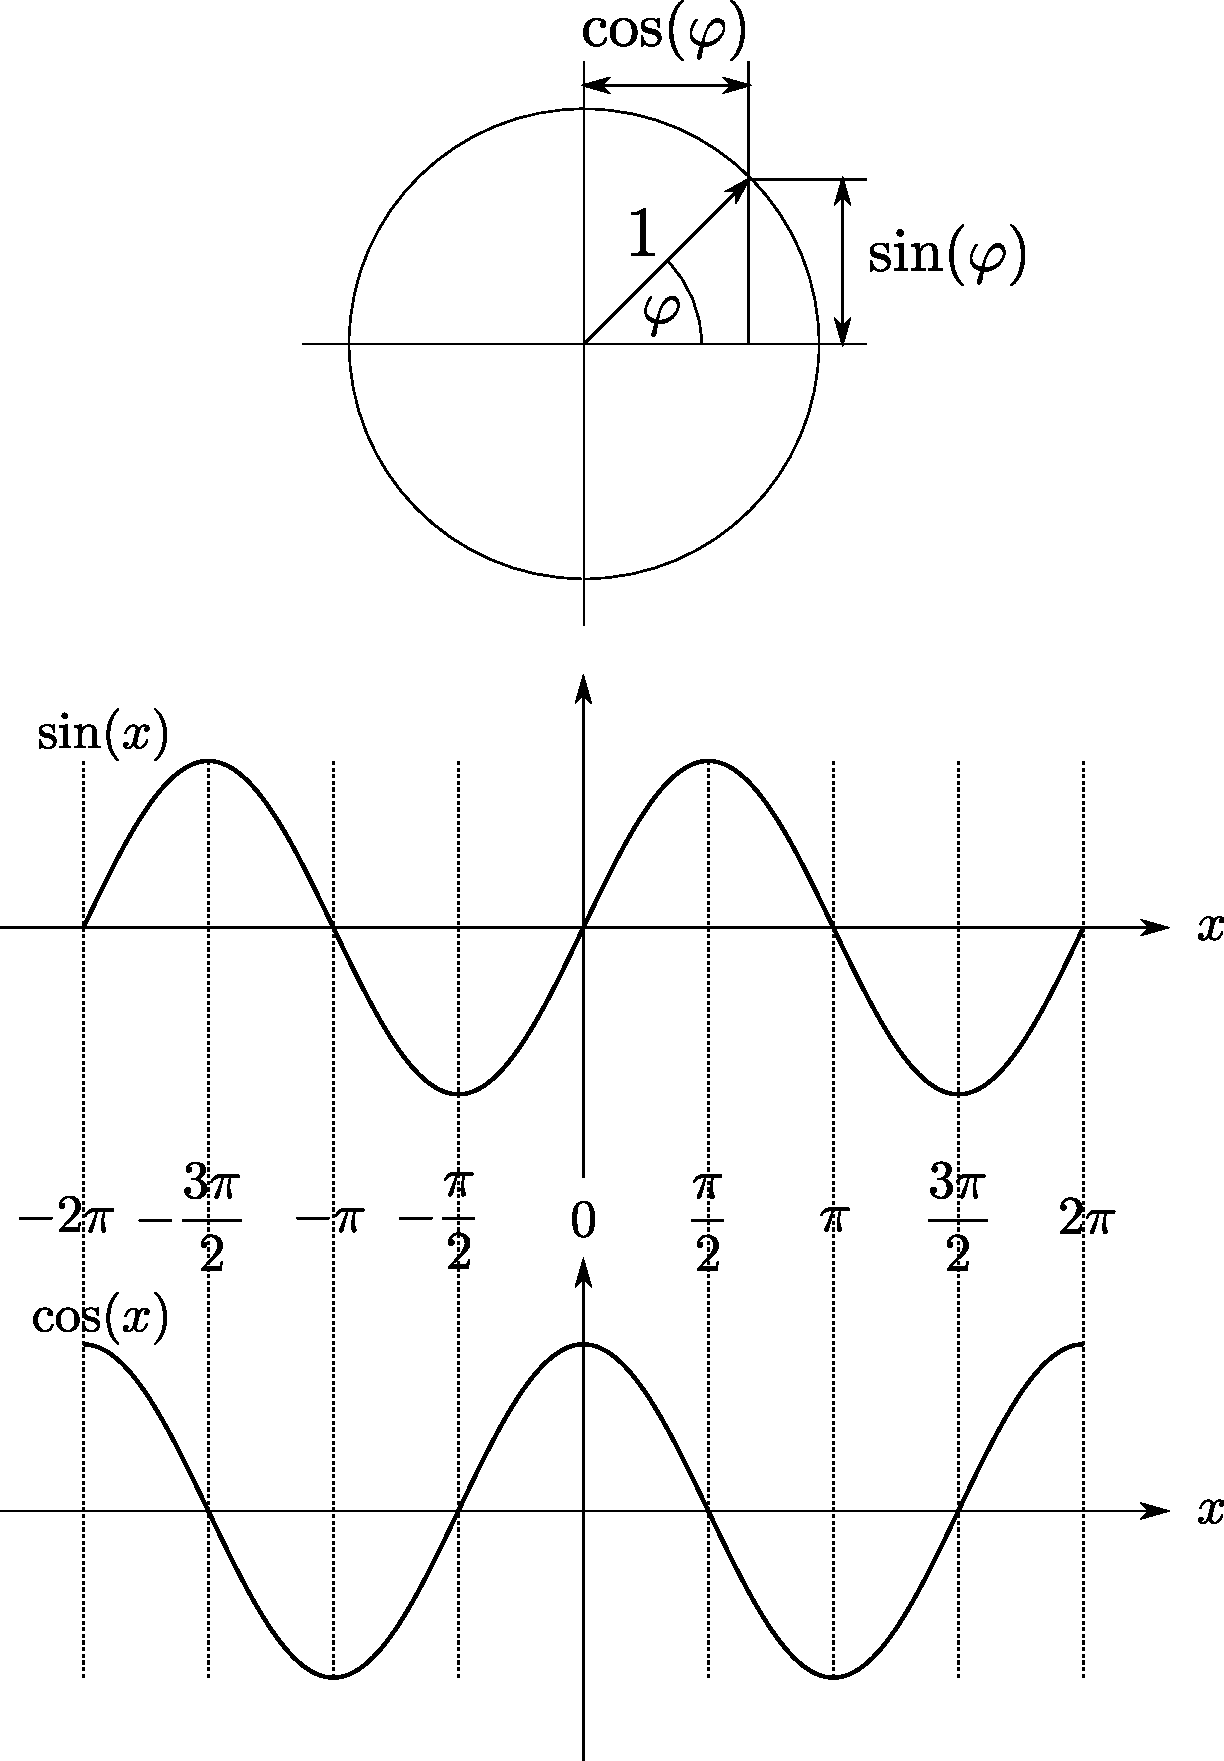
\includegraphics[width=0.8\textwidth]{einheitskreis.pdf}
\end{figure}

% \newpage
\noindent
$H$: Hypotenuse\\
$A$: Ankathete\\
$G$: Gegenkathete
\[ \boxed{\sin\alpha=\frac{G}{H}} \quad \boxed{\cos\alpha=\frac{A}{H}} 
\quad \boxed{\tan\alpha=\frac{G}{A}} \quad \boxed{\cot\alpha=\frac{A}{G}} \]
\[ \boxed{\sin x = \sqrt{1-\cos^2x} = \sqrt{\frac{\tan^2x}{1+\tan^2x}}} \]
\[ \boxed{\cos x = \sqrt{1-\sin^2x} = \sqrt{\frac{1}{1+\tan^2x}}} \]
\[ \boxed{\tan x = \frac{\sin x}{\sqrt{1-\sin^2x}} 
= \frac{\sqrt{1-\cos^2x}}{\cos x} = \frac{\sin x}{\cos x}} \]
\[ \boxed{\sin^2 x + \cos^2 x = 1} \]

\subsubsection{Additionstheoreme}
\[ \boxed{\sin(x+y) = \sin(x) \cdot cos(y) + \cos(x) \cdot \sin(y) }\]
\[ \boxed{\sin(2x) = 2 \cdot \sin(x) \cdot \cos(x) }\]
\[ \boxed{\cos(x+y) = \cos(x) \cdot \cos(y) - \sin(x) \cdot \sin(y) }\]
\[ \boxed{\cos(2x) = \cos^2(x) - \sin^2(x) = 2 \cdot \cos^2(x) - 1 }\]

\subsection{Spezielle Werte der Winkelfunktionen} \label{tab:spez-winkel}
% \begin{tabular}{|l|c|c|c|c|c|}
% \hline              & 0°$ = 0$ & 30°$ = \frac{\pi}{6}$ & 45°$ = \frac{\pi}{4}$ & 60°$ = \frac{\pi}{3}$ & 90°$ = \frac{\pi}{2}$ \\
% \hline $f\left(x\right)=\sin x$ & $0$ & $\frac{1}{2}$ & $\frac{1}{2}\sqrt{2}$ & $\frac{1}{2}\sqrt{3}$ & $1$ \\
% \hline $f\left(x\right)=\cos x$ & $1$ & $\frac{1}{2}\sqrt{3}$ & $\frac{1}{2}\sqrt{2}$ & $\frac{1}{2}$ & $0$ \\
% \hline $f\left(x\right)=\tan x$ & $0$ & $\frac{1}{3}\sqrt{3}$ & $1$ & $\sqrt{3}$ & nicht def. \\
% \hline $f\left(x\right)=\cot x$ & nicht def. & $\sqrt{3}$ & $1$ & $\frac{1}{3}\sqrt{3}$ & $0$ \\
% \hline \end{tabular}

% \begin{tabular}{|l||r|r|r|r|}
% \hline $\varphi$                    &          $\sin(\varphi)$&          $\cos(\varphi)$&          $\tan(\varphi)$&          $\cot(\varphi)$\\
% \hline $0^\circ=0$                  &                      $0$&                      $1$&                      $0$&          nicht definiert\\
% \hline $30^\circ=\frac{\pi}{6}$     &            $\frac{1}{2}$&    $\frac{1}{2}\sqrt{3}$&    $\frac{1}{3}\sqrt{3}$&               $\sqrt{3}$\\
% \hline $45^\circ=\frac{\pi}{4}$     &    $\frac{1}{2}\sqrt{2}$&    $\frac{1}{2}\sqrt{2}$&                      $1$&                      $1$\\
% \hline $60^\circ=\frac{\pi}{3}$     &    $\frac{1}{2}\sqrt{3}$&            $\frac{1}{2}$&               $\sqrt{3}$&    $\frac{1}{3}\sqrt{3}$\\
% \hline $90^\circ=\frac{\pi}{2}$     &                      $1$&                      $0$&          nicht definiert&                      $0$\\
% \hline $120^\circ=\frac{2\pi}{3}$   &    $\frac{1}{2}\sqrt{3}$&           $-\frac{1}{2}$&              $-\sqrt{3}$&   $-\frac{1}{3}\sqrt{3}$\\
% \hline $135^\circ=\frac{3\pi}{4}$   &    $\frac{1}{2}\sqrt{2}$&   $-\frac{1}{2}\sqrt{2}$&                     $-1$&                     $-1$\\
% \hline $150^\circ=\frac{5\pi}{6}$   &            $\frac{1}{2}$&   $-\frac{1}{2}\sqrt{3}$&   $-\frac{1}{3}\sqrt{3}$&              $-\sqrt{3}$\\
% \hline $180^\circ=\pi$              &                      $0$&                     $-1$&                      $0$&          nicht definiert\\
% \hline $210^\circ=\frac{7\pi}{6}$   &           $-\frac{1}{2}$&   $-\frac{1}{2}\sqrt{3}$&    $\frac{1}{3}\sqrt{3}$&               $\sqrt{3}$\\
% \hline $225^\circ=\frac{5\pi}{4}$   &   $-\frac{1}{2}\sqrt{2}$&   $-\frac{1}{2}\sqrt{2}$&                      $1$&                      $1$\\
% \hline $240^\circ=\frac{4\pi}{3}$   &   $-\frac{1}{2}\sqrt{3}$&           $-\frac{1}{2}$&               $\sqrt{3}$&    $\frac{1}{3}\sqrt{3}$\\
% \hline $270^\circ=\frac{3\pi}{2}$   &                     $-1$&                      $0$&          nicht definiert&                      $0$\\
% \hline $300^\circ=\frac{5\pi}{3}$  &   $-\frac{1}{2}\sqrt{3}$&            $\frac{1}{2}$&              $-\sqrt{3}$&   $-\frac{1}{3}\sqrt{3}$\\
% \hline $315^\circ=\frac{7\pi}{4}$   &   $-\frac{1}{2}\sqrt{2}$&    $\frac{1}{2}\sqrt{2}$&                     $-1$&                     $-1$\\
% \hline $330^\circ=\frac{11\pi}{6}$  &           $-\frac{1}{2}$&    $\frac{1}{2}\sqrt{3}$&   $-\frac{1}{3}\sqrt{3}$&              $-\sqrt{3}$\\
% \hline $360^\circ=2 \pi$            &                      $0$&                      $1$&                      $0$&          nicht definiert\\
% \hline\end{tabular}

% \[ \begin{array}{|l||r|r|r|r|}
% \hline \varphi                    &          \sin(\varphi)&          \cos(\varphi)&          \tan(\varphi)&          \cot(\varphi)\\
% \hline 0^\circ=0                  &                      0&                      1&                      0& \text{nicht definiert}\\
% \hline 30^\circ=\frac{\pi}{6}     &            \frac{1}{2}&    \frac{1}{2}\sqrt{3}&    \frac{1}{3}\sqrt{3}&               \sqrt{3}\\
% \hline 45^\circ=\frac{\pi}{4}     &    \frac{1}{2}\sqrt{2}&    \frac{1}{2}\sqrt{2}&                      1&                      1\\
% \hline 60^\circ=\frac{\pi}{3}     &    \frac{1}{2}\sqrt{3}&            \frac{1}{2}&               \sqrt{3}&    \frac{1}{3}\sqrt{3}\\
% \hline 90^\circ=\frac{\pi}{2}     &                      1&                      0& \text{nicht definiert}&                      0\\
% \hline 120^\circ=\frac{2\pi}{3}   &    \frac{1}{2}\sqrt{3}&           -\frac{1}{2}&              -\sqrt{3}&   -\frac{1}{3}\sqrt{3}\\
% \hline 135^\circ=\frac{3\pi}{4}   &    \frac{1}{2}\sqrt{2}&   -\frac{1}{2}\sqrt{2}&                     -1&                     -1\\
% \hline 150^\circ=\frac{5\pi}{6}   &            \frac{1}{2}&   -\frac{1}{2}\sqrt{3}&   -\frac{1}{3}\sqrt{3}&              -\sqrt{3}\\
% \hline 180^\circ=\pi              &                      0&                     -1&                      0& \text{nicht definiert}\\
% \hline 210^\circ=\frac{7\pi}{6}   &           -\frac{1}{2}&   -\frac{1}{2}\sqrt{3}&    \frac{1}{3}\sqrt{3}&               \sqrt{3}\\
% \hline 225^\circ=\frac{5\pi}{4}   &   -\frac{1}{2}\sqrt{2}&   -\frac{1}{2}\sqrt{2}&                      1&                      1\\
% \hline 240^\circ=\frac{4\pi}{3}   &   -\frac{1}{2}\sqrt{3}&           -\frac{1}{2}&               \sqrt{3}&    \frac{1}{3}\sqrt{3}\\
% \hline 270^\circ=\frac{3\pi}{2}   &                     -1&                      0& \text{nicht definiert}&                      0\\
% \hline 300^\circ=\frac{5\pi}{3}   &   -\frac{1}{2}\sqrt{3}&            \frac{1}{2}&              -\sqrt{3}&   -\frac{1}{3}\sqrt{3}\\
% \hline 315^\circ=\frac{7\pi}{4}   &   -\frac{1}{2}\sqrt{2}&    \frac{1}{2}\sqrt{2}&                     -1&                     -1\\
% \hline 330^\circ=\frac{11\pi}{6}  &           -\frac{1}{2}&    \frac{1}{2}\sqrt{3}&   -\frac{1}{3}\sqrt{3}&              -\sqrt{3}\\
% \hline 360^\circ=2 \pi            &                      0&                      1&                      0& \text{nicht definiert}\\
% \hline\end{array} \]

\[ \boxed{\begin{array}{rclcccc}
\rowcolor{white} \multicolumn{3}{c}{\varphi}  &          \sin(\varphi)&          \cos(\varphi)&          \tan(\varphi)&          \cot(\varphi)\\
\rowcolor{white} \lbrack^\circ\rbrack & &\lbrack\text{rad}\rbrack\qquad&\qquad\qquad\qquad&\qquad\qquad\qquad&\qquad\qquad\qquad&\qquad\qquad\qquad\\
\rowcolor{lgray}-180^\circ&=&-\pi             &                      0&                     -1&                      0&          \text{n. def}\\
\rowcolor{white}-150^\circ&=&-\frac{5\pi}{6}  &           -\frac{1}{2}&   -\frac{1}{2}\sqrt{3}&    \frac{1}{3}\sqrt{3}&               \sqrt{3}\\
\rowcolor{lgray}-135^\circ&=&-\frac{3\pi}{4}  &   -\frac{1}{2}\sqrt{2}&   -\frac{1}{2}\sqrt{2}&                      1&                      1\\
\rowcolor{white}-120^\circ&=&-\frac{2\pi}{3}  &   -\frac{1}{2}\sqrt{3}&           -\frac{1}{2}&               \sqrt{3}&    \frac{1}{3}\sqrt{3}\\
\rowcolor{lgray} -90^\circ&=&-\frac{\pi}{2}   &                     -1&                      0&          \text{n. def}&                      0\\
\rowcolor{white} -60^\circ&=&-\frac{\pi}{3}   &   -\frac{1}{2}\sqrt{3}&            \frac{1}{2}&              -\sqrt{3}&   -\frac{1}{3}\sqrt{3}\\
\rowcolor{lgray} -45^\circ&=&-\frac{\pi}{4}   &   -\frac{1}{2}\sqrt{2}&    \frac{1}{2}\sqrt{2}&                     -1&                     -1\\
\rowcolor{white} -30^\circ&=&-\frac{\pi}{6}   &           -\frac{1}{2}&    \frac{1}{2}\sqrt{3}&   -\frac{1}{3}\sqrt{3}&              -\sqrt{3}\\
\rowcolor{lgray} 0^\circ  &=&0                &                      0&                      1&                      0&          \text{n. def}\\
\rowcolor{white} 30^\circ &=&\frac{\pi}{6}    &            \frac{1}{2}&    \frac{1}{2}\sqrt{3}&    \frac{1}{3}\sqrt{3}&               \sqrt{3}\\
\rowcolor{lgray} 45^\circ &=&\frac{\pi}{4}    &    \frac{1}{2}\sqrt{2}&    \frac{1}{2}\sqrt{2}&                      1&                      1\\
\rowcolor{white} 60^\circ &=&\frac{\pi}{3}    &    \frac{1}{2}\sqrt{3}&            \frac{1}{2}&               \sqrt{3}&    \frac{1}{3}\sqrt{3}\\
\rowcolor{lgray} 90^\circ &=&\frac{\pi}{2}    &                      1&                      0&          \text{n. def}&                      0\\
\rowcolor{white} 120^\circ&=&\frac{2\pi}{3}   &    \frac{1}{2}\sqrt{3}&           -\frac{1}{2}&              -\sqrt{3}&   -\frac{1}{3}\sqrt{3}\\
\rowcolor{lgray} 135^\circ&=&\frac{3\pi}{4}   &    \frac{1}{2}\sqrt{2}&   -\frac{1}{2}\sqrt{2}&                     -1&                     -1\\
\rowcolor{white} 150^\circ&=&\frac{5\pi}{6}   &            \frac{1}{2}&   -\frac{1}{2}\sqrt{3}&   -\frac{1}{3}\sqrt{3}&              -\sqrt{3}\\
\rowcolor{lgray} 180^\circ&=&\pi              &                      0&                     -1&                      0&          \text{n. def}\\
\rowcolor{white} 210^\circ&=&\frac{7\pi}{6}   &           -\frac{1}{2}&   -\frac{1}{2}\sqrt{3}&    \frac{1}{3}\sqrt{3}&               \sqrt{3}\\
\rowcolor{lgray} 225^\circ&=&\frac{5\pi}{4}   &   -\frac{1}{2}\sqrt{2}&   -\frac{1}{2}\sqrt{2}&                      1&                      1\\
\rowcolor{white} 240^\circ&=&\frac{4\pi}{3}   &   -\frac{1}{2}\sqrt{3}&           -\frac{1}{2}&               \sqrt{3}&    \frac{1}{3}\sqrt{3}\\
\rowcolor{lgray} 270^\circ&=&\frac{3\pi}{2}   &                     -1&                      0&          \text{n. def}&                      0\\
\rowcolor{white} 300^\circ&=&\frac{5\pi}{3}   &   -\frac{1}{2}\sqrt{3}&            \frac{1}{2}&              -\sqrt{3}&   -\frac{1}{3}\sqrt{3}\\
\rowcolor{lgray} 315^\circ&=&\frac{7\pi}{4}   &   -\frac{1}{2}\sqrt{2}&    \frac{1}{2}\sqrt{2}&                     -1&                     -1\\
\rowcolor{white} 330^\circ&=&\frac{11\pi}{6}  &           -\frac{1}{2}&    \frac{1}{2}\sqrt{3}&   -\frac{1}{3}\sqrt{3}&              -\sqrt{3}\\
\rowcolor{lgray} 360^\circ&=&2 \pi            &                      0&                      1&                      0&          \text{n. def}\\
\end{array}} \]

\newpage
\subsection{Quadratische Gleichung}
\[ \boxed{f(x) = a \cdot x^2 + b \cdot x + c} \]
\[ \boxed{x_{1,2}=\frac{-b\pm\sqrt{b^2-4ac}}{2a}} \]

\subsection{Kubische Gleichung}
Für kubische Gleichungen gibt es keine Lösungsformel. \\
Wenn der konstante Teil 0 ist, kann x ausgeklammert werden. 
\[ \boxed{\begin{array}{l}
ax^3 + bx^2 + cx = 0 \\
x(ax^2 + bx + c) = 0 \\
\rightarrow x_1 = 0 \\
ax^2 + bx + c = 0 \\
\rightarrow x_{2,3} = \frac{-b\pm\sqrt{b^2-4ac}}{2a}
\end{array}} \]

\ifti
\subsubsection{Vorsicht beim TI-89}
Wird beim TI-89 $y = x \cdot (\ldots)$ eingegeben, muss \verb!y=x*(...)! 
eingegeben werden. \verb!x(...)! wird vom Taschenrechner als Funktion 
interpretiert. 
\fi

\ifnspire
\subsubsection{Vorsicht beim TI-Nspire}
Wird beim TI-Nspire $y = x \cdot (\ldots)$ eingegeben, muss \verb!y=x*(...)! 
eingegeben werden. \verb!x(...)! wird vom Taschenrechner als Funktion 
interpretiert. 
\fi

\subsection{Faktorisieren}
In einigen Fällan ist es einfacher, ein Polynom zu faktorisieren. Das ist 
im Besonderen der Fall, wenn die binomischen Formeln angewendet werden können. 
Dabei wird der Term in ein Produkt aus Elementen der Form $(x+a)$ aufgeteilt. 
Jeder dieser Terme kann mit 0 gleichgesetzt werden und liefert somit jeweils 
eine der Lösungen. \\
Beispiel: \\
$x^2 + (a + b) \cdot x + a \cdot b = 0 $ \\
$\Rightarrow (x + a) \cdot (x + b) = 0$ \\
$\Rightarrow (x + a) =0, \quad (x + b) = 0$ \\
$\rightarrow x_1 = -a, \quad x_2 = -b$

\ifti
\subsubsection{Faktorisieren mit dem TI-89}
Soll ein Term der Form $x^3 - ax$ faktorisiert werden, kann es vorkommen, dass 
man ein Ergebnis der Form $x(x^2 - a)$ erhält. Damit der Taschenrechner nach 
$x(x-\sqrt{a})(x+\sqrt(a))$ faktorisiert, kann beim Befehl \verb!factor! als 
zweites Argument die Variable, nach der faktorisiert werden soll, übergeben 
werden. \\
$\rightarrow$ \verb!factor(x^3-a,x)!
\fi

\ifnspire
\subsubsection{Faktorisieren mit dem TI-Nspire}
Soll ein Term der Form $x^3 - ax$ faktorisiert werden, kann es vorkommen, dass 
man ein Ergebnis der Form $x(x^2 - a)$ erhält. Damit der Taschenrechner nach 
$x(x-\sqrt{a})(x+\sqrt(a))$ faktorisiert, kann beim Befehl \verb!factor! als 
zweites Argument die Variable, nach der faktorisiert werden soll, übergeben 
werden. \\
$\rightarrow$ \verb!factor(x^3-a,x)!
\fi

\subsection{Binomische Formeln}
Erste Binomische Formel: 
\[ \boxed{(a + b)^2 = a^2 + 2 \cdot a \cdot b + b^2} \]Zweite Binomische Formel: 
\[ \boxed{(a - b)^2 = a^2 - 2 \cdot a \cdot b + b^2} \]Dritte Binomische Formel: 
\[ \boxed{(a + b) \cdot (a - b) = a^2 - b^2} \]

\subsection{Verkettete Funktionen}
\[ \boxed{(f \circ g)(x) := f(g(x))} \]

\subsection{Grenzwerte}
\[ \boxed{\lim\limits_{x \to x_0}(f_1(x) + f_2(x)) 
= \lim\limits_{x \to x_0}(f_1(x)) + \lim\limits_{x \to x_0}(f_2(x))} \]
\[ \boxed{\lim\limits_{x \to x_0}(f_1(x) - f_2(x)) 
= \lim\limits_{x \to x_0}(f_1(x)) - \lim\limits_{x \to x_0}(f_2(x))} \]
\[ \boxed{\lim\limits_{x \to x_0}(f_1(x) \cdot f_2(x)) 
= \lim\limits_{x \to x_0}(f_1(x)) \cdot \lim\limits_{x \to x_0}(f_2(x))} \]
\[ \boxed{\lim\limits_{x \to x_0}\left(\frac{f_1(x)}{f_2(x)}\right) 
= \frac{\lim\limits_{x \to x_0}(f_1(x))}{\lim\limits_{x \to x_0}(f_2(x))}} \]
\[ \boxed{\lim\limits_{x \to x_0}(c \cdot f_1(x)) 
= c \cdot \lim\limits_{x \to x_0}(f_1(x))} \]
\[ \boxed{\lim\limits_{x \to x_0}\left(c^{(f_1(x))}\right) 
= c^{\left(\lim\limits_{x \to x_0}(f_1(x))\right)}} \]
\[ \boxed{\lim\limits_{x \to x_0}\left((f_1(x))^n\right) 
= \left(\lim\limits_{x \to x_0}(f_1(x))\right)^n} \]
\[ \boxed{\lim\limits_{x \to x_0}\left(\sqrt[n]{(f_1(x))}\right) 
= \sqrt[n]{\lim\limits_{x \to x_0}(f_1(x))}} \]
\[ \boxed{\lim\limits_{x \to x_0}\left(\log{(f_1(x))}\right) 
= \log{\lim\limits_{x \to x_0}(f_1(x))}} \]

\subsection{Berechnung von Grenzwerten}
Um Grenzwerte zu ermitteln muss der Ausdruck so angepasst werden, dass 
eindeutig bestimmt werden kann, was sich daraus ergibt.
Dies wird durch Anwenden der zuvor aufgezeigten Rechenreglen erreicht.\\\\
Bsp.: $ \quad \quad \lim\limits_{n \rightarrow \infty} 
\left( \dfrac{\alpha \cdot n^2}{n^2-1} \right) $ \\\\
Um den Grenzwert zu ermitteln muss der Ausdruck erweitert werden und zwar so, 
dass
\begin{itemize}
\item der Term äquivalent bleibt
\item Variabeln des Indizes entfallen
\end{itemize}
Um die geforderten Bedingungen zu erfüllen wird der Term durch den reziproken 
Wert des Indizes mit der höchsten Potenz (im Zähler!) erweitert. In diesem Fall 
mit $\frac{1}{n^2}$. 
Eine weitere Regel besagt, dass konstante Faktoren vorangenommen werden können.
Nun sieht es wie folgt aus:\\\\
\indent \indent \indent $ \alpha \lim\limits_{n \rightarrow \infty} 
    \left( \dfrac{\frac{1}{n^2} \cdot (n^2) }{ \frac{1}{n^2} \cdot (n^2 -1) } 
    \right)  $\\\\\\
Vereinfacht man diesen Ausdruck durch elementare Algebra so erhält man: \\\\
\indent \indent \indent $ \alpha \lim\limits_{n \rightarrow \infty} 
\left( \dfrac{1}{1-
\smash{\underbrace{\frac{1}{n^2}}_0 } \vphantom{\dfrac{1}{n^2}} } \right)$\\\\\\
Der Audruck $\frac{1}{n^2}$ geht für $n \rightarrow \infty$ zu $0$. Daraus 
ergibt sich das folgende:\\\\\\
\indent \indent \indent $ \alpha \cdot 1 = \alpha $
\ifti
\subsubsection{Berechnung von Grenzwerten mit dem TI-89}\label{subsubsec:limti}
%limit($a_n$, $n$, $\infty)$
\verb?limit(EXP,VAR,POINT[,DIRECTION])?\\\\
\begin{tabular}{@{}lll}
\verb|EXP|	& Ausdruck	& bezeichnet den Term \\
\verb|VAR|	& Variable	& bezeichnet die Variable \\
\verb|POINT|	& Punkt		& bezeichnet den Variablenwert \\
\verb|DIRECTION|& Richtung 	& bezeichnet die Richtung \\
		&		& $\searrow$~~~~von oben: 1 \\
		&		& $\nearrow$~~~~von unten: -1 \\
\end{tabular}\\\\
Bsp.: \verb| limit((x^2-2)/(x-2),x,2,-1)| \\
\indent\indent erzeugt die Ausgabe $\mathtt{ \lim\limits_{x \rightarrow 2^-} 
(\dfrac{x^2-2}{x-2}) \quad = \quad - \infty } $
\fi
\iftiboth
\newpage
\fi
\ifnspire
\subsubsection{Berechnung von Grenzwerten mit dem TI-Nspire}
\label{subsubsec:limnspire}
\[ \lim\limits_{\boxed{n}\to\boxed{\infty}^{\boxed{d}}}(\boxed{a_n}) \]\\
\begin{tabular}{@{}llp{6cm}}
$\boxed{a_n}$    & Ausdruck & bezeichnet den Term \\
$\boxed{n}$      & Variable & bezeichnet die Variable \\
$\boxed{\infty}$ & Punkt    & bezeichnet den Variablenwert \\
$\boxed{d}$      & Richtung & bezeichnet die Richtung \\
                 &          & $\searrow$ : von oben: + \\
                 &          & $\nearrow$ : von unten: - \\
		 &          & Wenn keine Richtung gefordert ist, kann dieses Feld leer 
         gelassen werden. 
\end{tabular}\\\\
Dieses Symbol findet man nach Druck auf die Taste $\boxed{\boxed{|\boxed{}|
\left\{\frac{\boxed{}}{\boxed{}}\right.}}$
\fi

\subsubsection{L'Hopital}
Die Regel von L'Hopital besagt, dass wenn man einen Grenzwert der Form 
\[ \lim\limits_{x \rightarrow x_0} \frac{f(x)}{g(x)} \Rightarrow 
\lim\limits_{x \rightarrow x_0} f(x) = \lim\limits_{x \rightarrow x_0} g(x) = 0 
\Rightarrow \lim\limits_{x \rightarrow x_0} \frac{0}{0} \] hat, kann der 
Grenzwert auch über die Ableitungen ermittelt werden, falls der Grenzwert 
existiert.
Erhält man wieder einen unbestimmten Ausdruck, so kann erneut die Regel von 
L'Hopital angewendet werden (dies kann man so oft wie nötig wiederholen).
\[ \boxed{ \lim\limits_{x \rightarrow x_0} \frac{f(x)}{g(x)} 
= \lim\limits_{x \rightarrow x_0} \frac{f'(x)}{g'(x)} \quad} \quad 
\text{falls Bedingungen erfüllt sind!}\]

\subsection{Hyperbolicus}
\[ \boxed{\sinh(x) =: \frac{1}{2}\left(e^x - e^{-x} \right) }\]
\[ \boxed{\cosh(x) =: \frac{1}{2}\left(e^x + e^{-x} \right) }\]

\subsection{Fakultät}
\[ \boxed{K! = 1 \cdot 2 \cdot 3\cdot \ldots \cdot K} \qquad \boxed{0! := 1} \]
\[ \boxed{(K + 1)! = 1  \cdot 2 \cdot \ldots \cdot K \cdot (K + 1) = (K + 1) 
\cdot K!} \]
\[ \boxed{(K - 1)! = 1  \cdot 2 \cdot \ldots \cdot (K - 1) = 1  \cdot 2 \cdot 
\ldots \cdot (K - 1) \cdot \frac{K}{K} = \frac{K!}{K}} \]
\subsubsection{Einige Fakultäten}
\[ \boxed{\begin{array}{rcr}
\rowcolor{white}  0!&=&1\\
\rowcolor{lgray}  1!&=&1\\
\rowcolor{white}  2!&=&2\\
\rowcolor{lgray}  3!&=&6\\
\rowcolor{white}  4!&=&24\\
\rowcolor{lgray}  5!&=&120\\
\rowcolor{white}  6!&=&720\\
\rowcolor{lgray}  7!&=&5'040\\
\rowcolor{white}  8!&=&40'320\\
\rowcolor{lgray}  9!&=&362'880\\
\rowcolor{white} 10!&=&3'628'800\\
\rowcolor{lgray} 11!&=&39'916'800\\
\rowcolor{white} 12!&=&479'001'600\\
\rowcolor{lgray} 13!&=&6'227'020'800\\
\rowcolor{white} 14!&=&87'178'291'200\\
\rowcolor{lgray} 15!&=&1'307'674'368'000\\
\rowcolor{white} 16!&=&20'922'789'888'000\\
\rowcolor{lgray} 17!&=&355'687'428'096'000\\
\rowcolor{white} 18!&=&6'402'373'705'728'000\\
\rowcolor{lgray} 19!&=&121'645'100'408'832'000\\
\rowcolor{white} 20!&=&2'432'902'008'176'640'000\\
\end{array}}\]

% \[ \boxed{\begin{spreadtab}{{array}{lrlcr}}
% @\rowcolor{white}& 0&@!&@=&1 \\
% @\rowcolor{lgray}& \STcopy{v}{b1+1}&@!&@=&\STcopy{v}{e1*b2}\\
% @\rowcolor{white}& &@!&@=& \\
% @\rowcolor{lgray}& &@!&@=& \\
% @\rowcolor{white}& &@!&@=& \\
% @\rowcolor{lgray}& &@!&@=& \\
% @\rowcolor{white}& &@!&@=& \\
% @\rowcolor{lgray}& &@!&@=& \\
% @\rowcolor{white}& &@!&@=& \\
% @\rowcolor{lgray}& &@!&@=& \\
% @\rowcolor{white}& &@!&@=& \\
% @\rowcolor{lgray}& &@!&@=& \\
% @\rowcolor{white}& &@!&@=& \\
% @\rowcolor{lgray}& &@!&@=& \\
% @\rowcolor{white}& &@!&@=& \\
% @\rowcolor{lgray}& &@!&@=& \\
% @\rowcolor{white}& &@!&@=& \\
% @\rowcolor{lgray}& &@!&@=& \\
% @\rowcolor{white}& &@!&@=& \\
% @\rowcolor{lgray}& &@!&@=& \\
% @\rowcolor{white}& &@!&@=& \\
% \end{spreadtab}}\]

\newpage
\subsection{Pascal'sches Dreieck}
Um ein Pascal'sches Dreieck zu zeichnen beginnt man mit einer "'1"'. Diagonal 
rechts und links unterhalb werden wieder zwei Zahlen gezeichnet. So wird das 
Dreieck Reihe für Reihe aufgebaut. Jede Zahl wird dabei aus der Summe der 
beiden Zahlen links und rechts oberhalb berechnet. Stellen an denen keine Zahl 
steht werden als Null gezählt. 
\begin{figure}[h!]
	\centering
	\begin{tikzpicture}
	\foreach \n in {0,...,6} {
		  \foreach \k in {0,...,\n} {
		      \node at (\k-\n/2,-\n) {$\binomialCoefficient{\n}{\k}$};
		        }
		}
	\end{tikzpicture}	
\caption{Pascal'sches Dreieck bis zum Grad 6}
\end{figure}

\subsubsection*{Formel}
\[ (x+y)^n = ax^ny^0 + bx^{n-1}y^1 + cx^{n-2}y^2 + dx^{n-3}y^3 + \ldots + ux^{1}y^{n-1} + vx^0y^n \]
Die Konstanten $a,b,c\ldots$ sind die Koeffizienten aus dem Pascalschen Dreieck (Zeilen) und $n$ ist 
der Grad. Bei einen Binom vierten Grades $(x+y)^4$ wären dies 
\[ n=4 \] und \[ a=1, b=4, c=6, d=4, e=1 \]
und somit 
\[ (x+y)^4 = 1x^4y^0 + 4x^3y^1 + 6x^2y^2 + 4x^1y^3 + 1x^0y^4 \]



% coding:utf-8
\section{Darstellung von Funktionen}
\subsection{Polares Koordinatensystem}
Eine Funktion kann auch im Polaren Koordinatensystem definiert werden. 
Dabei wird jeder Punkt durch den Abstand zur Ordinate und den Winkel zur x-Achse definiert. 

\begin{figure}[h!]
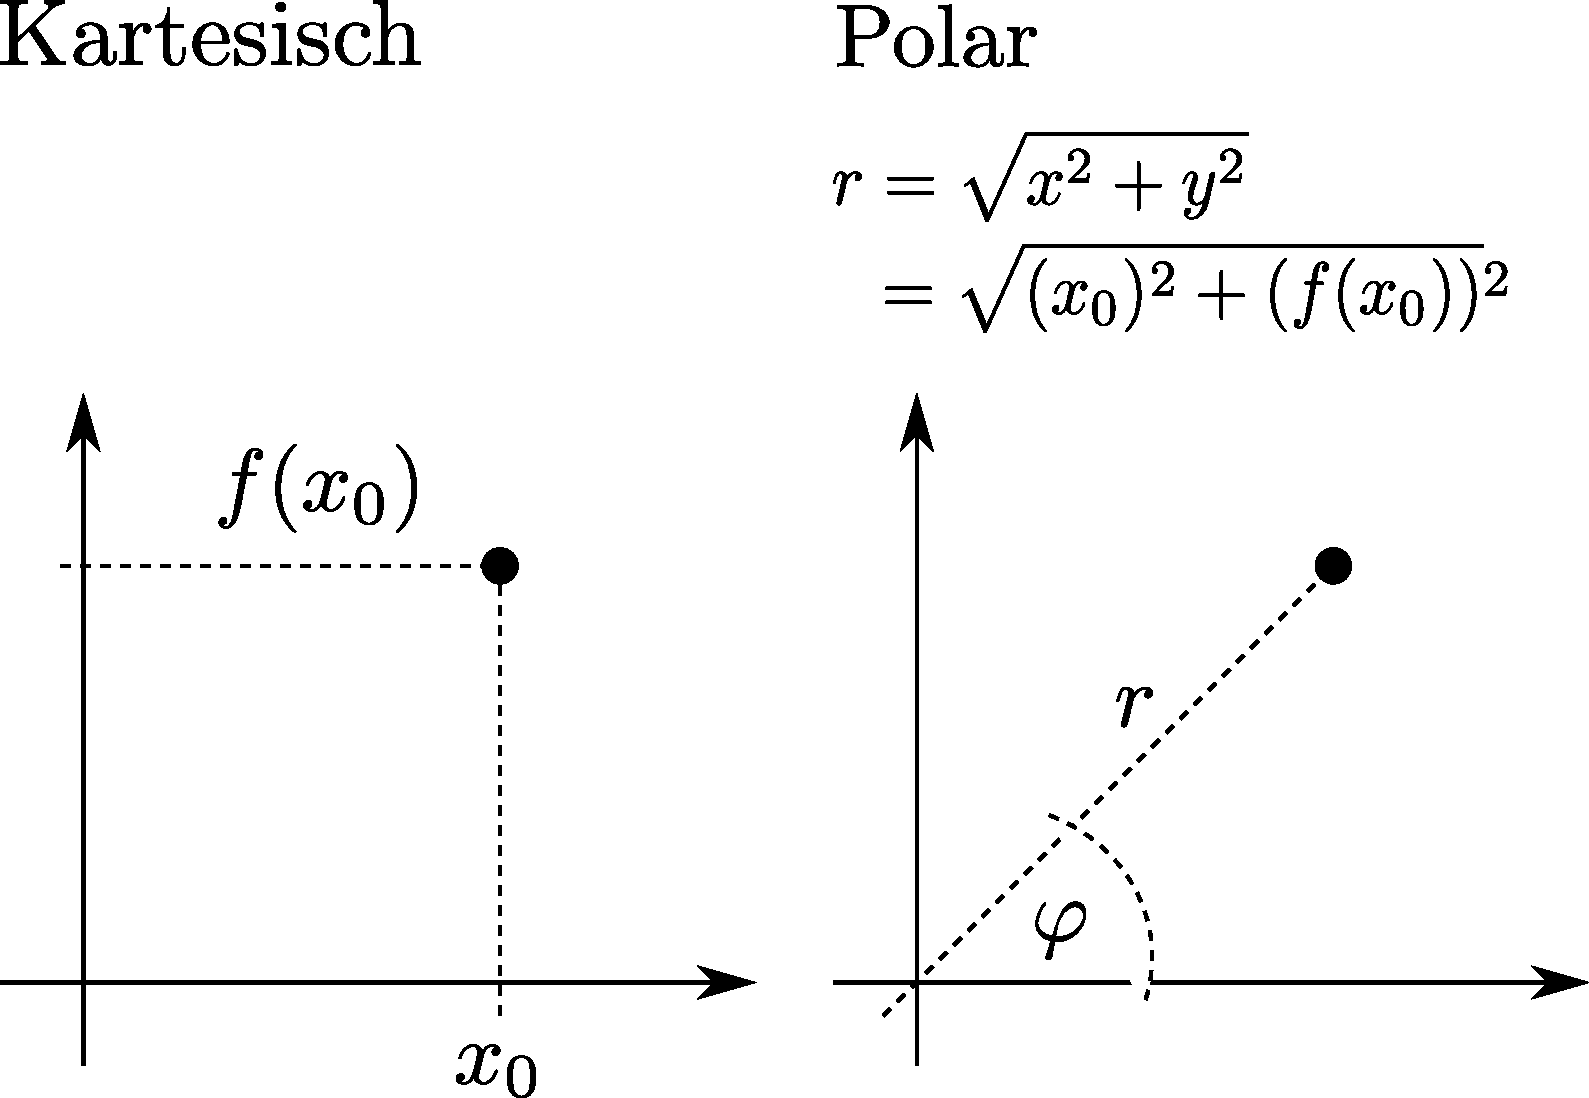
\includegraphics[height=1\textwidth,angle=270]{polar.pdf}
\end{figure}

%\begin{figure}[h!]
%\includegraphics[height=1\textwidth,angle=270]{polar_2.pdf}
%\end{figure}

\subsection{Umrechnung Kartesisch $\rightarrow$ Polar}
\[ \boxed{r = \sqrt{x^2 + y^2}} \]
\[ \boxed{\varphi = \arctan\left(\frac{y}{x}\right)} \]

\subsection{Umrechnung Polar $\rightarrow$ Kartesisch}
\[ \boxed{x = r \cdot \cos{\varphi}} \]
\[ \boxed{y = r \cdot \sin{\varphi}} \]

\subsection{Parameterdarstellung}
Bei der Paramaterdarstellung wird jeder Punkt durch die x- und die y-Koordinate definiert. 
\[ \boxed{f(t) = \left(\begin{matrix} x(t)\\ y(t) \end{matrix}\right)} \]


\chapter{Vektorgeometrie}
\section{Vektorgeometrie in der Ebene}

\subsection{Anstand zweier Puntke}
\[ \boxed{ \overline{P_1 P_2} = \sqrt{ (x_2 - x_1)^2 + (y_2 - y_1)^2 } } \]

\subsection{Geradengleichungen}

\subsubsection{Normalform (explizite Form)}
\[ \boxed{ g: y= mx + q }\]
\[ \boxed{ \text{Steigung } m = \frac{y_2 - y_1}{x_2 - x_1} = \frac{\Delta y}{\Delta x}  = tan \varphi } \]

\subsubsection{Koordinatenform (implizite Form)}
\[ \boxed{ g: ax + by + c = 0 } \]

\subsubsection{Achsenabschnittsform}
\[ \boxed{ g: \frac{x}{p} + \frac{y}{q} = 1 } \]

\subsubsection{Hesse'sche Normalform}
\[ \boxed{ g:  \frac{ax + by + c}{\sqrt{ a^2 + b^2 } } = 0 }  \]

\subsubsection{Parameterform}
\[ \boxed{ 
    g: \vec{r} = \vec{r_0} + t \cdot \vec{a}  = 
      \left( 
	\begin{array}{cc} 
	  x_0 \\ y_0
	\end{array}
      \right)
      + t \cdot 
      \left( 
	\begin{array}{cc} 
	  a_x \\ a_y
	\end{array}
      \right)  
   }
\]


\subsection{Normalenvektor}
Der Normalenvektor ist ein Vektor, welcher senkrecht auf einem anderen Vektor bzw. einer Geraden liegt. Hier im Beispiel in welchem $ \vec{n} \bot g(x)$
\[ \boxed{ \vec{n} = 
      \left( 
	\begin{array}{cc} 
	  n_x \\ n_y
	\end{array}
      \right)
      =
      \left( 
	\begin{array}{cc} 
	  a \\ b
	\end{array}
      \right)
      =
      \left( 
	\begin{array}{cc} 
	  -a_y \\ a_x
	\end{array}
      \right)
} \]
\noindent
Der Richtungsvektor von $g(x)$ ist 
$  
      \left( 
	\begin{array}{cc} 
	  a_x \\ a_y
	\end{array}
      \right)
      \Rightarrow 
      \left( 
	\begin{array}{cc} 
	  -a_y \\ a_x
	\end{array}
      \right)
      = \vec{n}
$.

\subsection{Abstand Punkt zu Gerade}
Für eine Gerade $g: ax + by + c = 0$ und einen Punkt $P_1 (x_1 | y_1)$ gilt:
\[ \boxed{ d = \left| \frac{ax_1 + by_1 + c}{\sqrt{a^2 + b^2}} \right| } \]

\subsection{Schnittwinkel zwischen Geraden}
Für den spitzen Schnittwinkel $\varphi$ zwischen den Geraden 

$g_1: y = m_1x + q_1$ und $g_2: y = m_2x + q_2$ gilt:
\[ \boxed{ tan\varphi = \left| \frac{m_2 - m_1}{1 + m_1 \cdot m_2} \right| } \\ \text{für } \varphi \neq 90^{\circ} \]

\[ \boxed{ g_1 || g_2 \Leftrightarrow m_1 = m_2 \text{und } g_1 \bot g_2 \Leftrightarrow m_2 = - \frac{1}{m_1} } \\ \text{für } m_1 \neq 0 \]

\section{Vektorgeometrie im Raum}

\subsection{Ortsvektor}
Ein Ortsvektor beschreibt den Vektor vom Urspung des Koordinatensystems $O(0|0|0)$ zu einem beliebigen Punkt $P(x|y|z)$.
\[	\boxed{ \vec{r} = \overrightarrow{OP} = x\vec{e_x} + y\vec{e_y} + z\vec{e_z} :=
	\left( 
	  \begin{array}{ccc} 
	    x \\ y \\ z
	  \end{array}
	\right) }
\]
\noindent
Die Vektoren $\vec{e_x},\vec{e_y},\vec{e_z}$ sind die Einheitsvektoren des Koordinatensystems (meist einfach 1 ohne Einheit).
\subsection{Länge eines Ortsvektors (Betrag)}
\[ \boxed{ |\vec{r}| = r = \sqrt{x^2 + y^2 1 z^2} } \]


\chapter{Folgen und Reihen}
% coding:utf-8

%----------------------------------------
%FOSAMATH, a LaTeX-Code for a mathematical summary for basic analysis
%Copyright (C) 2013, Daniel Winz, Ervin Mazlagic, Adrian Imboden, Philipp Langer

%This program is free software; you can redistribute it and/or
%modify it under the terms of the GNU General Public License
%as published by the Free Software Foundation; either version 2
%of the License, or (at your option) any later version.

%This program is distributed in the hope that it will be useful,
%but WITHOUT ANY WARRANTY; without even the implied warranty of
%MERCHANTABILITY or FITNESS FOR A PARTICULAR PURPOSE.  See the
%GNU General Public License for more details.
%----------------------------------------


% coding:utf-8
\section{Folgen}
$a_1$ (bzw. $a_0$) ist das erste Glied einer Folge\\
$a_n$ ist das $n$-te Glied einer Folge

\subsection{Form}
Eine Folge kann drei spezielle Formen annehmen. Für $(a_n)_{n \in \mathbb{N}}$ 
gilt die Folge je nach dem als
\subsubsection*{monoton wachsend}
$ \boxed{ a_{n+1} \geq a_n \quad \forall \quad n \in \mathbb{N} } $ Bsp.: $a_n 
= 2^n$, $a_{n+1} = 2^{n+1}$
\subsubsection*{monoton fallend}
$ \boxed{ a_{n+1} \leq a_n \quad \forall \quad n \in \mathbb{N} } $ Bsp.: $a_n 
= \frac{1}{n}$, $a_{n+1} = \frac{1}{n+1}$
\subsubsection*{alternierend}
$ \boxed{ a_{n+1} \cdot a_n < 0 } $ Bsp.: $a_n := (-2)^n$, $a_{n+1} 
= (-2)^{n+1} \cdot (-2)^n = (-2)^{2n+1}$\\\\
Bei den monoton wachsend/fallenden Folgen kann noch weiter unterschieden werden 
zwischen streng monoton und einfach monoton. Streng monoton bedeutet dann, dass 
$a_n \neq a_{n+1}$ wobei das bei einfach monotonen der Fall sein kann 
(vgl.~\ref{subsec:monotonie}).
\subsection{rekursive Darstellung}
Bei der rekursiven Darstellung wird eine Folge durch einen Startwert und eine 
Abbildungsvorschrift dargestellt. \\
\[ \boxed{ \begin{matrix}
\text{Startwert} & f(1) = a_1 \\
\text{Vorschrift} & F(f(1), f(2), \ldots, f(n)) := f(n + 1) = a_{n + 1}
\end{matrix}} \]

\subsection{arithmetische Folgen}
$d$ ist die Differenz zwischen zwei benachbarten Gliedern\\
\[ \boxed{d = a_{n+1} - a_n} \]
\[ \boxed{a_{n+1} = a_n + d} \]
\[ \boxed{ \begin{matrix} 
a_0 :& a_n =& a_0 + n \cdot d \\
a_1 :& a_n =& a_1 + (n - 1)d 
\end{matrix}}\]

\subsection{geometrische Folgen}
$q$ ist der Quotient von zwei benachbarten Gliedern\\
\[ \boxed{\frac{a_{n+1}}{a_n} = q} \]
\[ \boxed{a_{n+1} = a_n \cdot q} \]
\[ \boxed{\begin{array}{ll}
a_0 :& a_n = q^{n} a_0\\
a_1 :& a_n = q^{n-1} a_1
\end{array}} \]

\ifti
\subsubsection{Folgen mit dem TI-89}
%seq($a_n$, Variable, $n_1$, $n_2$)\\\\
\verb{seq(EXP,VAR,LOW,HIGH[,STEP]){\\\\
\begin{tabular}{@{}lll}
EXP	& Ausdruck	& bezeichnet den Term \\
VAR 	& Variable	& bezeichnet die inkrementierte Variabel \\
LOW	& untere Grenze	& Anfangspunkt der Inkrementierung \\
HIGH	& obere Grenze	& Endpunkt der Inkrementierung \\
STEP	& n-Schritte	& Zeigt Resultate mit n-ten Schritt
\end{tabular}\\\\
Bsp.: \verb{seq(1/x,x,1,10,5){ erzeugt die Ausgabe \verb?{1   1/6}?
\fi
\ifnspire
\subsubsection{Folgen mit dem TI-Nspire}
seq($a_n$, Variable, $n_1$, $n_2$)\\\\
\begin{tabular}{@{}ll}
$a_n$    & Formel für die Berechnung des n-ten Gliedes\\
Variable & Variable in der Formel\\
$n_1$    & erstes zu berechnendes Glied\\
$n_2$    & letztes zu berechnendes Glied
\end{tabular}
\fi

\subsection{Konvergenz von Folgen}
Eine Folge ist konvergent, wenn der Grenzwert der Folge eine reelle Zahl ist
\[ \boxed{\lim\limits_{n \to \infty} a_n = a \quad a \in \mathbb{R}}\]

\subsubsection{Rechenregeln}
$ a_n \xrightarrow[\rightarrow \infty]{} a $, 
$ b_n \xrightarrow[n \rightarrow \infty]{} b $
\[ \boxed{ a_n + b_n \xrightarrow[]{n \rightarrow \infty} a + b } \]
\[ \boxed{ a_n - b_n \xrightarrow[]{n \rightarrow \infty} a - b } \]
\[ \boxed{ a_n \cdot b_n \xrightarrow[]{n \rightarrow \infty} a \cdot b } \]
\[ \boxed{ \alpha \cdot a_n \xrightarrow[]{n \rightarrow \infty} \alpha \cdot a, 
\quad \alpha \in \mathbb{R} } \]
\[ \boxed{ \frac{a_n}{b_n} \xrightarrow[]{n \rightarrow \infty} \frac{a}{b}, 
\quad \text{falls} \quad b_n \neq 0 \quad \forall \quad n \in \mathbb{N} } \]

\ifti
\subsubsection{Konvergenz von Folgen mit dem TI-89}
Für die Berechnung von Grenzwerten mit dem TI-89 siehe \ref{subsubsec:limti}. 
\fi
\ifnspire
\subsubsection{Konvergenz von Folgen mit dem TI-Nspire}
Für die Berechnung von Grenzwerten mit dem TI-Nspire siehe 
\ref{subsubsec:limnspire}. 
\fi

% coding:utf-8
\section{Reihen}
$S_n$ ist die Summe aller Glieder von $a_1$ bis $a_n$. 
\[ \boxed{S_n = \sum_{k=1}^{n} a_k = a_1 + a_2 + a_3 \cdots + a_n} \]

\subsection{arithmetische Reihe}
\[ \boxed{S_n = \left(n + 1\right)\left(a_0 + d \frac{n}{2}\right) = \left(n + 1\right) \frac{a_0 + a_n}{2}} \]

\subsection{geometrische Reihe}
\[ \boxed{\text{Für } q \neq 1: \quad S_n = a_1 \left(  \frac{q^n - 1}{q - 1} \right) = a_1 \left(  \frac{1 - q^n}{1 - q} \right)} \]

\[ \boxed{\begin{array}{ll}
a_0 :& S_n = a_0 \cdot \dfrac{1-q^{n+1}}{1-q} \\ 
& \\
a_1 :& S_n = a_1 \cdot \dfrac{1-q^n}{1-q}
\end{array}} \]

\[ \boxed{\text{Für } q = 1: \quad S_n = a_1 \left(1+1^1 + 1^2 + \ldots + 1^{n-1}\right) = a_1 n} \]
Unendliche geometrische Reihe
\[ \boxed{\text{Für } |q| < 1: S = \lim_{n \rightarrow \infty} S_n = \frac{a_1}{1 - q}} \] 
%Um das $n$-te Glied einer geometrischen Reihen zu berechnen gilt:\\
%$ q = \frac{a_n}{a_{n-1}} = \frac{a_{n-1}}{a_{n-2}} $ \\
%$ \Rightarrow  a_n = a_{(n-1)} \cdot q = a_{(n-2)} \cdot q^2 = a_{(n - (n-1))} \cdot q^{(n-1)} = a_1 \cdot q^{(n-1)} $
%\[ \boxed{ a_n = a_1 \cdot q^{n-1} } \]
%\[ \boxed{ a_{n+1} = a_1 \cdot q^n } \]
$a_1$ ist hier das erste Element der geometrischen Folge!

\subsection{Konvergenz}

\subsubsection*{Quotientenkriterium}
Um die Konvergenzfrage einer geometrischen Reihe zu klären betrachtet man
\[ \lim\limits_{n \rightarrow \infty} \left| \frac{a_{n+1}}{a_n} \right| = \lim\limits_{n \rightarrow \infty} \left| q \right| \]
Hierbei können drei verschiedene Ergebnisse entstehen:
\[ \boxed{\begin{array}{ll}
|q| < 1 & \text{die Reihe konvergiert} \\
|q| > 1 & \text{die Reihe divergiert} \\
|q| = 1 & \text{keine Aussage möglich}
\end{array}} \]
Dies wird oft als Quotientenkriterium bezeichnet.

\subsubsection*{Wurlzelkrierium}
Eine weitere Methode zur Klärung der Konvergenzfrage liefert das so genannte Wurzelkriterium.
\[ \lim\limits_{n \rightarrow \infty} \left( |a_k| \right)^{\frac{1}{n}} = q\]
Daraus können wie beim Quotientenkriterium drei Fälle eintreten:
\[ \boxed{\begin{array}{ll}
|q| < 1 & \text{die Reihe konvergiert} \\
|q| > 1 & \text{die Reihe divergiert} \\
|q| = 1 & \text{keine Aussage möglich} 
\end{array}} \]


\ifti
\subsection{Reihen mit dem TI89 berechnen}
$\sum$\verb{(Ausdruck,Variable,untere Grenze, obere Grenze){ \\
$\sum$\verb{(EXP,VAR,LOW,HIGH){ \\\\
\begin{tabular}{lll}
EXP  & Ausdruck      & bezeichnet den Term der die Reihe beschreibt \\
VAR  & Variable      & bezeichnet die inkrementierte Variable \\
LOW  & untere Grenze & Anfangspunkt der Inkrementierung \\
HIGH & obere Grenze  & Endpunkt der Inkrementierung \\
\end{tabular}
\fi


\chapter{Differenzieren}
% coding:utf-8
\section{Ableitungsregeln}

\subsection{Grundoperationen}

\subsubsection{Summenregel}
\[ \boxed{ (f(x) + g(x))' = f'(x) + g'(x) } \]
\[ \text{Wichtig: Ableitung einer konstanten Funktion ist Null! } \]
\[ \Rightarrow (f(x) + c)' = f'(x) \text{ für } c \in R \]

\subsubsection{Faktorregel}
\[ \boxed{ (c \cdot f(x))' = c \cdot f'(x) } \]
\[ \text{Ein konstanter Faktor bleiobt beim Differenzieren (Ableiten) erhalten!} \]

\subsubsection{Produkteregel}
\[ \boxed{ (f(x) \cdot g(x))' = f'(x) \cdot g(x) + f(x) \cdot g'(x) } \]

\subsubsection{Quotientenregel}
\[ \boxed{ \left( \frac{f(x)}{g(x)} \right) = \frac{ f'(x) \cdot g(x) - f(x) \cdot g'(x) }{ g^2(x) } } \\ \text{ gilt falls }g(x) \neq 0 \text{ !} \]

\subsubsection{Kettenregel}
\[ \boxed{ (f(g(x)))' = g'(x) \cdot f'(g(x)) } \]

\newpage

\subsection{Spezielle Regeln}

\subsubsection{Exponenten}
\[ \boxed{ (x^n)' = n\cdot x^{(n-1)} } \]
\[ \boxed{ (e^x)' = e^x } \]
\[ \boxed{ (e^{k\cdot x})' = k \cdot e^{k\cdot x} } \]
\[ \boxed{ (a^x)' = ln_a (a^x) } \]

\subsubsection{Logarithmen}
\[ \boxed{ (ln(x))' = \frac{1}{x} } \]  
% \[ \boxed{ (a_{log_x})' = \frac{1}{x \cdot ln(a)} } \]

\subsubsection{Trigonometrie}
\[ \boxed{ (sin(x))' = cos(x) } \]  
\[ \boxed{ (cos(x))' = -sin(x) } \] 
\[ \boxed{ (tan(x))' = \frac{1}{cos^2(x)} } \]  
\[ \boxed{ (cot(x))' = -\frac{1}{sin^2(x)} } \]

% coding:utf-8

%----------------------------------------
%FOSAMATH, a LaTeX-Code for a mathematical summary for basic analysis
%Copyright (C) 2013, Daniel Winz, Ervin Mazlagic, Adrian Imboden, Philipp Langer

%This program is free software; you can redistribute it and/or
%modify it under the terms of the GNU General Public License
%as published by the Free Software Foundation; either version 2
%of the License, or (at your option) any later version.

%This program is distributed in the hope that it will be useful,
%but WITHOUT ANY WARRANTY; without even the implied warranty of
%MERCHANTABILITY or FITNESS FOR A PARTICULAR PURPOSE.  See the
%GNU General Public License for more details.
%----------------------------------------

% coding:utf-8
\section{Kurvendiskussion}

\subsection{Tangentengleichnung}
\label{subsec:tangentengleichung}
\[ \boxed{T(x) = f'(x_0)(x - x_0) + f(x_0)} \]

\subsection{Normale zur Tangente}
\[ \boxed{ T(x) = \frac{-1}{f'(x_0)} \cdot (x-x_0) + f(x_0) } \]

\subsection{Steigen und Fallen}

\[ \boxed{ \begin{array}{lll}
f'(x) \geq 0 \text{ auf } I & \Rightarrow  
& f \text{ ist monoton wachsend in $I$} \\
f'(x) \leq 0 \text{ auf } I & \Rightarrow  
& f \text{ ist monoton fallend in $I$} \\
f'(x) > 0 \text{ auf } I & \Rightarrow  
& f \text{ ist streng monoton wachsend in $I$} \\
f'(x) < 0 \text{ auf } I & \Rightarrow  
& f \text{ ist streng monoton fallend in $I$}
\end{array} } \]

\noindent
$I$ entspricht einem Intervall! Dies bedeutet, ist $f'(x)$ über den gesamten 
Bereich immer $\geq 0$ so ist $f$ monoton wachsend. Ist $f'(x)$ über den 
gesamten Bereich $\leq 0$ so ist sie monoton fallend.

\subsection{Krümmungsverhalten}

\[ \boxed{ \begin{matrix}
f''(x) > 0 \text{ auf } I & \Rightarrow  
& \text{ Kurve ist konvex bzw. linksgekrümmt} \\
f''(x) < 0 \text{ auf } I & \Rightarrow  
& \text{ Kurve ist konkav bzw. rechtsgekrümmt}
\end{matrix} } \]

\subsection{Extremum}
Ein Extremum ist ein Punkt, zu welchem die Ableitung $0$ ergibt.
Solch ein Extremum kann ein Maximum oder Minimum sein.
Zusätzlich ist zu definieren ob es sich um ein lokales oder globales Extremum 
handelt.

\[ \boxed{ \begin{matrix}
f'(x_0) = 0 \land f''(x_0) < 0 & \Rightarrow & \text{lokales Maximum in $x_0$}\\
f'(x_0) = 0 \land f''(x_0) > 0 & \Rightarrow & \text{lokales Minimum in $x_0$} 
\end{matrix} } \]

\subsection{Wendepunkt}
Als Wendepukt bezeichnet man jene Stelle, an welcher die Krümmung der Funktion 
wechselt (konkav zu konvex und umgekehrt).
Im Wendepunkt ist die Steigung jeweils von beiden Seiten aus betrachtet 
(d.h aus $x_0 > 0$ und $x_0<0$) extremal.

\subsubsection{Notwendiges Kriterium}
\[ \boxed{ \begin{matrix}
f''(x_0) = 0 & \Rightarrow & \text{Wendepunkt in $x_0$}
\end{matrix} } \]

\subsubsection{Hinreichendes Kriterium}
\[ \boxed{ \begin{matrix}
f''(x_0) = 0 \land f'''(x_0) \neq 0 & \Rightarrow & \text{Wendepunkt in $x_0$}
\end{matrix} } \]
Achtung: Ist die dritte Ableitung 0, so kann an dieser Stelle trotzdem ein 
Wendepunkt sein. 

\subsection{Sattelpunkt}
Ein Sattelpunkt ist ein Wendepunkt mit horizontaler Wendetangente.

\[ \boxed{ \begin{matrix}
f'(x_0) =  f''(x_0) = 0 \land f'''(x_0) \neq 0 & \Rightarrow 
& \text{Sattelpunkt in $x_0$}
\end{matrix} } \]

\begin{figure}[h!]
\centering
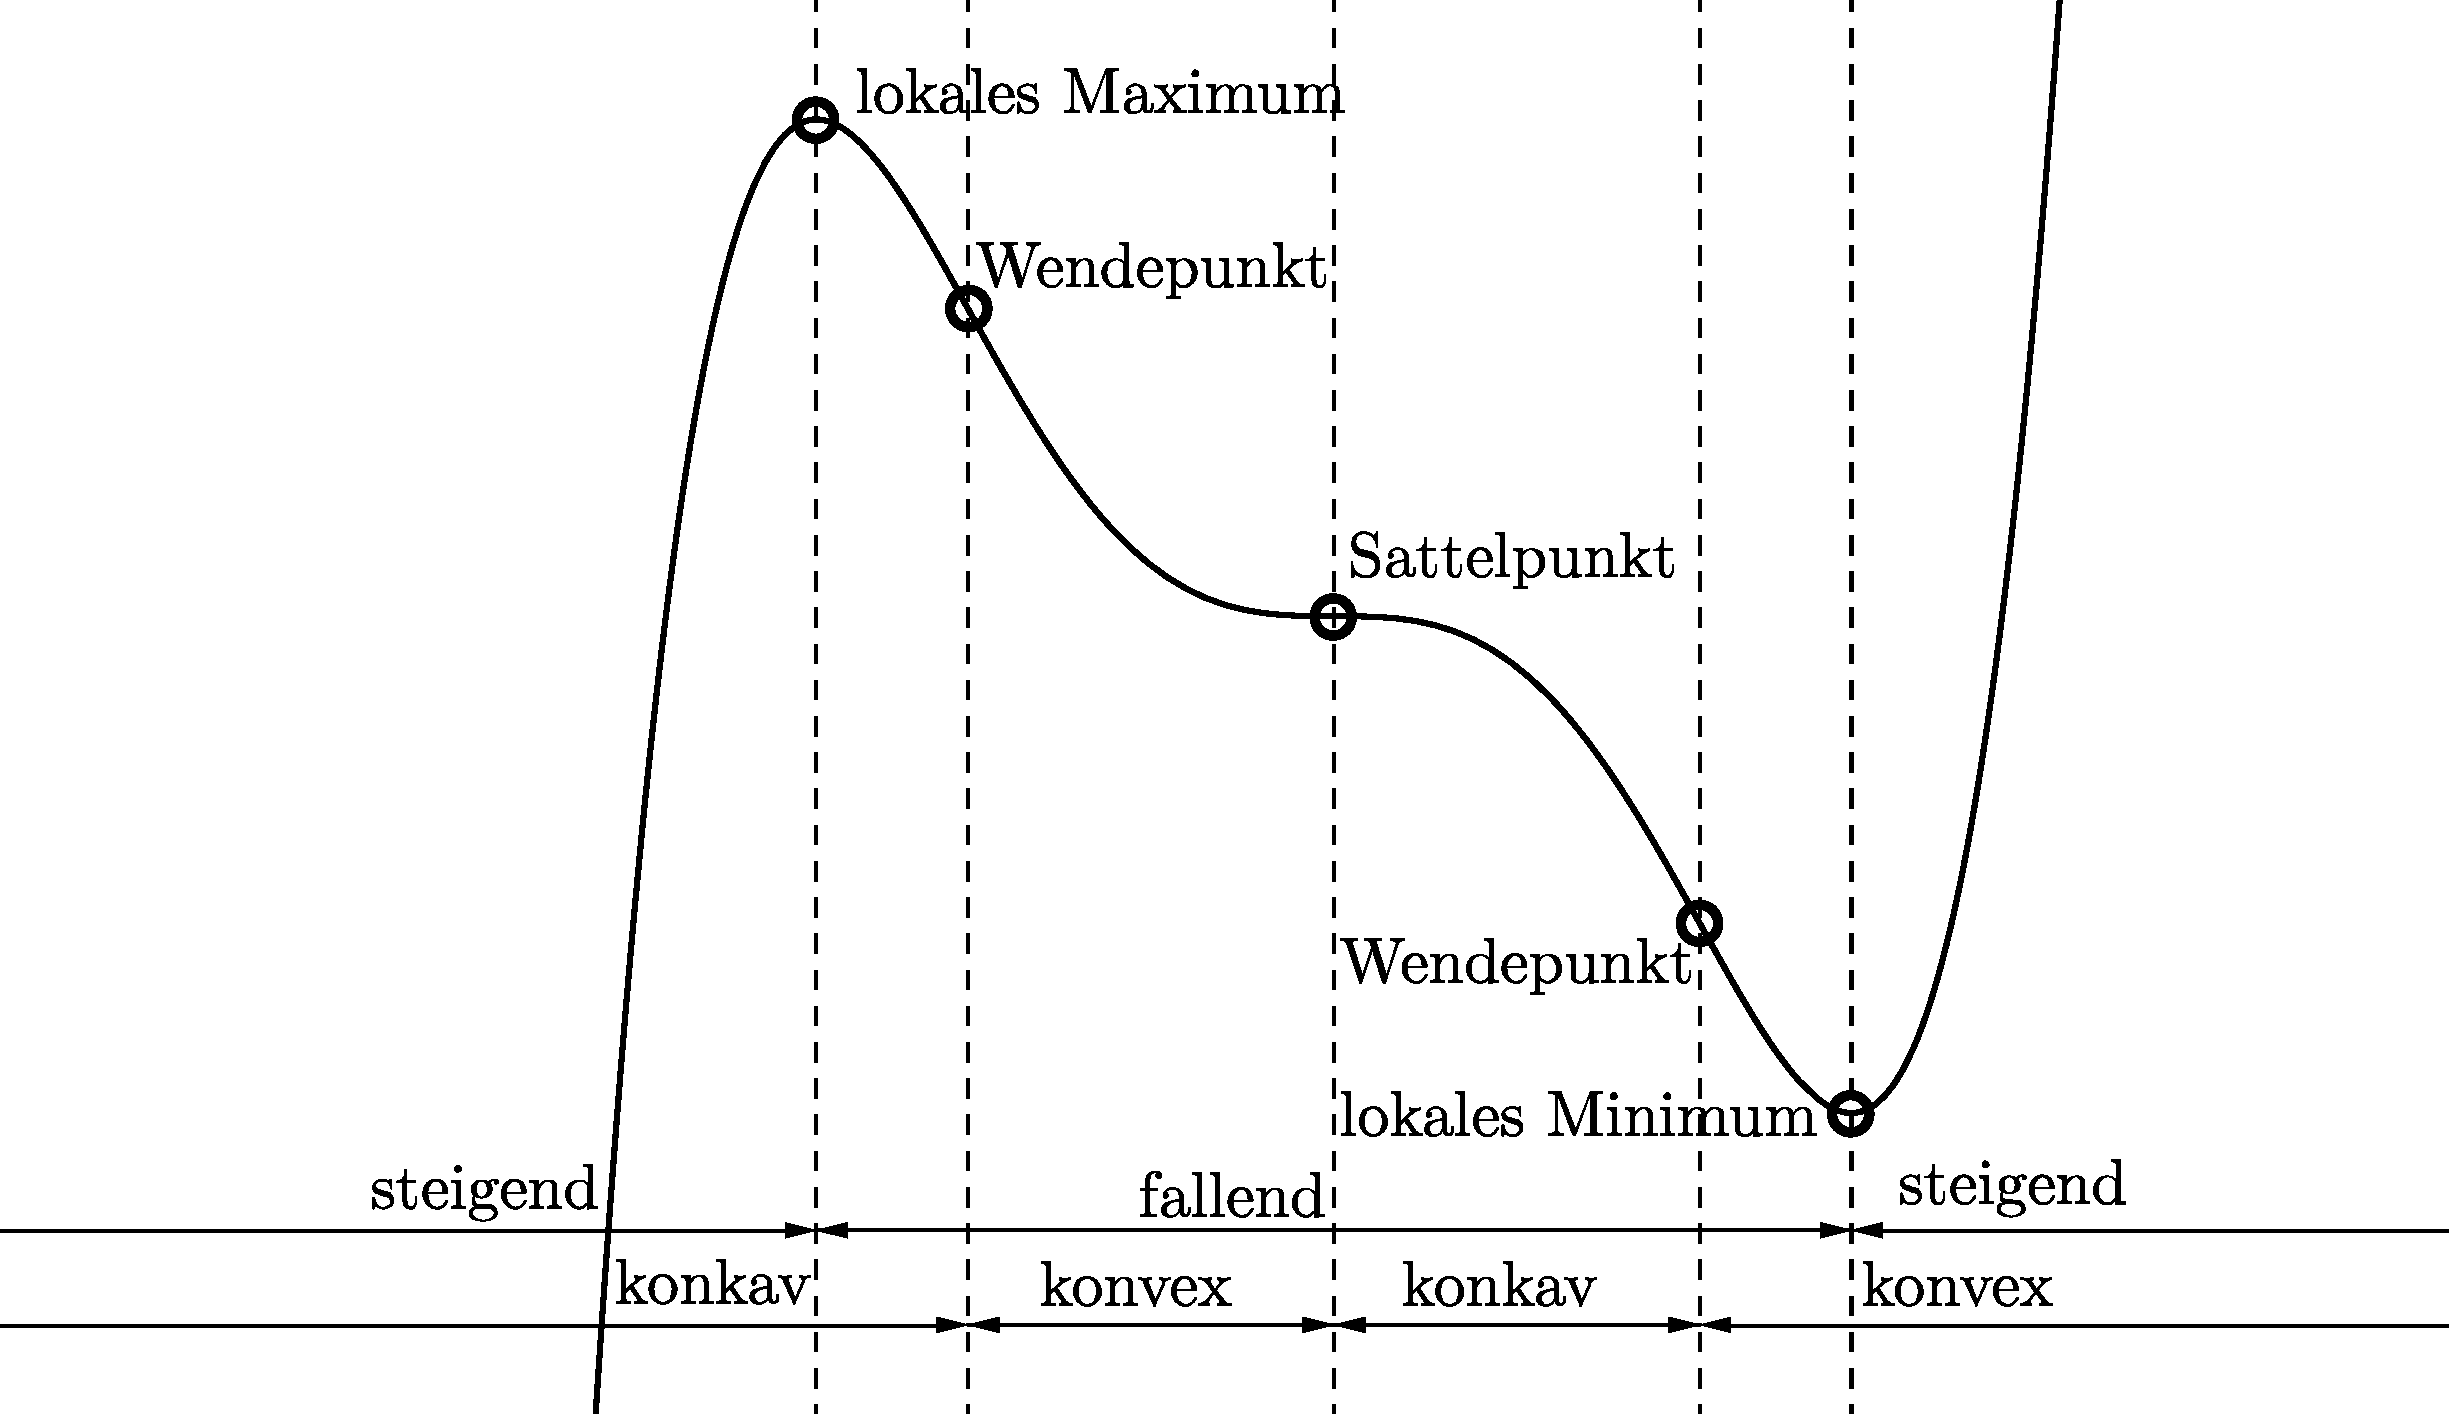
\includegraphics[width=0.88\textwidth]{kurvendiskussion.pdf}
\end{figure}
% coding:utf-8



%----------------------------------------

%FOSAMATH, a LaTeX-Code for a mathematical summary for basic analysis

%Copyright (C) 2013, Daniel Winz, Ervin Mazlagic, Adrian Imboden, Philipp Langer



%This program is free software; you can redistribute it and/or

%modify it under the terms of the GNU General Public License

%as published by the Free Software Foundation; either version 2

%of the License, or (at your option) any later version.



%This program is distributed in the hope that it will be useful,

%but WITHOUT ANY WARRANTY; without even the implied warranty of

%MERCHANTABILITY or FITNESS FOR A PARTICULAR PURPOSE.  See the

%GNU General Public License for more details.

%----------------------------------------


% coding:utf-8

\section{Krümmung}

Die Krümmung $\kappa$ misst wie stark eine Kurve $\gamma$ gekrümmt ist (vgl. Kreis hat eine konstante Krümmung).
Die Krümmung wird unterschieden in mittlere und momentane Krümmung.
\[ \begin{array}{ll}
	\text{mittlere}  & \dfrac{\Delta \alpha}{\Delta s} \\
	& \\
	\text{momentane} & \dfrac{\delta \alpha}{\delta s} \\
\end{array} \]

\[ \boxed{r(t) = \dfrac{1}{|\kappa(t)|} \quad \quad \text{bzw.} \quad \quad r(x) = \dfrac{1}{|\kappa(x)|} } \]
\[ \boxed{\kappa(x) = \frac{y''(x)}{(1 + y'(x)^2)^{\frac{3}{2}}} }\]

\[\boxed{\begin{array}{lllll} 
	\kappa (x) > 0 & \rightarrow & y''(x) \stackrel{!}{>} 0 & \rightarrow & y \text{ ist konvex} \\
	\kappa (x) < 0 & \rightarrow & y''(x) \stackrel{!}{<} 0 & \rightarrow & y \text{ ist konkav} \\
	\kappa (x) = 0 & \rightarrow & y''(x) = 0		& \xrightarrow[]{Achtung!} & \text{Wendepunkt!}
\end{array}}\]
\section{Scheitelpunkte}
Scheitelpunkte sind Stellen an denen die Krümmung maximal ist. 
Um diese zu berechnen muss die Krümmung $\kappa (x)$ abgeleitet und Null gesetzt werden.
\[ \kappa '(x) \stackrel{!}{=} 0  \]
\[ \boxed{\kappa '(x) = \dfrac{ y'''(x)(1+y'(x)^2)^{\frac{3}{2}} - y''(x) \frac{3}{2}(1+y'(x)^2)^{\frac{1}{2}} y''(x) 2y'(x) }{ (1+y'(x)^2)^3 } \stackrel{!}{=} 0 } \]


\chapter{Integral}
% coding:utf-8



%----------------------------------------

%FOSAMATH, a LaTeX-Code for a mathematical summary for basic analysis

%Copyright (C) 2013, Daniel Winz, Ervin Mazlagic, Adrian Imboden, Philipp Langer



%This program is free software; you can redistribute it and/or

%modify it under the terms of the GNU General Public License

%as published by the Free Software Foundation; either version 2

%of the License, or (at your option) any later version.



%This program is distributed in the hope that it will be useful,

%but WITHOUT ANY WARRANTY; without even the implied warranty of

%MERCHANTABILITY or FITNESS FOR A PARTICULAR PURPOSE.  See the

%GNU General Public License for more details.

%----------------------------------------


% coding:utf-8
\section{Integral}
\subsection{Riemann Integral}
\[ \boxed{A_n = \Delta x \sum_{i=0}^{n-1} f(x_i) \quad 
, \Delta x = \frac{b - a}{n} , x_i = i \Delta , I = [a,b]} \]
Riemann-Summe! \\
Falls diese Summe resp. Reihe konvergent ist, so schreibt man
\[ \boxed{\lim_{n \rightarrow \infty} A_n = \int_{a}^{b} f(x) d x \quad \text{Riemann Integral von f über I = [a,b]} } \]

\subsection{Integral für ein beliebiges Polynom}
\[ \boxed{\int x^n = \frac{x^{n + 1}}{n + 1}} \]

\section{Eigenschaften des bestimmten Integrals}

\subsection{Summenregel}
\[ \boxed{\int_a^b (f(x) + g(x)) dx = \int_a^b f(x) dx + \int_a^b g(x) dx} \]

\subsection{Faktorregel}
\[ \boxed{\int_a^b \alpha \cdot f(x) dx = \alpha \int_a^b f(x) dx \quad , \forall \alpha \in \mathbb{R}} \]

\subsection{Additivität des Integrals}
\[ \boxed{\int_a^b f(x) dx = \int_a^c f(x) dx + \int_c^b f(x) dx \quad , a \leq c \leq b} \]
\\
Es gilt für: 
\[ \boxed{\int_a^b x^n dx = \int_0^b x^n dx - \int_0^a x^n dx = \frac{b^{n+1} - a^{n+1}}{n + 1} \quad , n \neq -1} \]
\[ \boxed{n = 0: \quad \int_a^b x^0 dx = \int_a^b 1 dx = b - a} \]

% coding:utf-8
\section{Integrationsregeln}
\subsection{Partielles Integrieren}
\[ \boxed{\int f'(x) \cdot g(x) dx = f(x) \cdot g(x) - \int f(x) \cdot g'(x) dx} \]
\subsection{Substitutionsregel}
\[ \boxed{\int_{g(a)}^{g(b)} f(x) dx = \int_{a}^{b} g'(x) \cdot f(g(x)) dx} \]


\section{Volumen}
\subsectrion{Rotationsvolumen}
\[ \boxed{V_x = \pi \int_{x_1}^{x_2} f(x)^2 dx} \quad \text{Rotation um die y-Achse}\]
\[ \boxed{V_y = \pi \int_{y_1}^{y_2} f^{-1}(y)^2 dy \quad \text{Rotation um die x-Achse}} \]

% coding:utf-8
\section{Ableitungen und unbestimmte Integrale spezieller Funktionen}
Integrationskonstante C ist weggelassen\\\\
% \begin{tabular}{|c|c|c|}
% \hline \rule{80pt}{0pt} & \rule{80pt}{0pt} & \rule{80pt}{0pt} \\
% \textbf{$f'(x)$} & \textbf{$f(x)$} & \textbf{$\int f(x) dx$}\\&&\\
% \hline $0$ & $c \quad c \in \mathbb{R}$ & $cx$ \\
% \hline $c$ & $cx$ & $\frac{c}{2}x^2$ \\
% \hline $r \cdot x^{r-1}$ & $x^r \quad r \in \mathbb{R} \backslash \{-1\}$ & $\frac{x^{r+1}}{r+1}$ \\
% \hline $-\frac{1}{x^2} = -x^{-2}$ & $\frac{1}{x} = x^{-1}$ & $ln{|x|}$ \\
% \hline $\frac{1}{2\sqrt{x}} = \frac{1}{2}x^{-\frac{1}{2}}$ & $\sqrt{x} = x^{\frac{1}{2}}$ & $\frac{2}{3}x^{\frac{3}{2}}$ \\
% \hline $\cos x$ & $\sin x$ & $-\cos x$ \\
% \hline $-\sin x$ & $\cos x$ & $\sin x$ \\
% \hline $1 + \tan^2 x = \frac{1}{\cos^2 x}$ & $\tan x$ & $-\ln |\cos x|$ \\
% \hline $e^x$ & $e^x$ & $e^x$ \\
% \hline $c \cdot e^x$ & $e^{cx}$ & $\frac{1}{c} \cdot e^{cx}$ \\
% \hline $\ln a \cdot a^x$ & $a^x$ & $\frac{a^x}{\ln a}$ \\
% \hline $\frac{1}{x}$ & $\ln |x|$ & $x(ln |x| - 1)$ \\
% \hline $\frac{1}{ln a \cdot x}$ & $\log_a |x|$ & $\frac{x}{\ln a}(\ln |x| - 1) = x(\log_a |x| - \log_a e)$ \\
% \hline $\frac{1}{\sqrt{1 - x^2}}$ & $\arcsin x$ & $x \cdot \arcsin x + \sqrt{1 - x^2}$ \\
% \hline $-\frac{1}{\sqrt{1 - x^2}}$ & $\arccos x$ & $x \cdot \arccos x - \sqrt{1 - x^2}$ \\
% \hline $\frac{1}{1 + x^2}$ & $\arctan x$ & $x \cdot \arctan x - \frac{1}{2}\ln(1 + x^2)$ \\
% \hline \end{tabular}
% \\\\\\
\begin{equation*}
\begin{matrix}
f'(x) & f(x) & \int f(x) dx\\
0 & c \quad c \in \mathbb{R} & cx \\
c & cx & \frac{c}{2}x^2 \\
r \cdot x^{r-1} & x^r \quad r \in \mathbb{R} \backslash \{-1\} & \frac{x^{r+1}}{r+1} \\
-\frac{1}{x^2} = -x^{-2} & \frac{1}{x} = x^{-1} & ln{|x|} \\
\frac{1}{2\sqrt{x}} = \frac{1}{2}x^{-\frac{1}{2}} & \sqrt{x} = x^{\frac{1}{2}} & \frac{2}{3}x^{\frac{3}{2}} \\
\cos x & \sin x & -\cos x \\
-\sin x & \cos x & \sin x \\
1 + \tan^2 x = \frac{1}{\cos^2 x} & \tan x & -\ln |\cos x| \\
e^x & e^x & e^x \\
c \cdot e^x & e^{cx} & \frac{1}{c} \cdot e^{cx} \\
\ln a \cdot a^x & a^x & \frac{a^x}{\ln a} \\
\frac{1}{x} & \ln |x| & x(ln |x| - 1) \\
\frac{1}{ln a \cdot x} & \log_a |x| & \frac{x}{\ln a}(\ln |x| - 1) = x(\log_a |x| - \log_a e) \\
\frac{1}{\sqrt{1 - x^2}} & \arcsin x & x \cdot \arcsin x + \sqrt{1 - x^2} \\
-\frac{1}{\sqrt{1 - x^2}} & \arccos x & x \cdot \arccos x - \sqrt{1 - x^2} \\
\frac{1}{1 + x^2} & \arctan x & x \cdot \arctan x - \frac{1}{2}\ln(1 + x^2) \\
\end{matrix}
\end{equation*}

\chapter{Taylorreihen}
% coding:utf-8

%----------------------------------------
%FOSAMATH, a LaTeX-Code for a mathematical summary for basic analysis
%Copyright (C) 2013, Daniel Winz, Ervin Mazlagic, Adrian Imboden, Philipp Langer

%This program is free software; you can redistribute it and/or
%modify it under the terms of the GNU General Public License
%as published by the Free Software Foundation; either version 2
%of the License, or (at your option) any later version.

%This program is distributed in the hope that it will be useful,
%but WITHOUT ANY WARRANTY; without even the implied warranty of
%MERCHANTABILITY or FITNESS FOR A PARTICULAR PURPOSE.  See the
%GNU General Public License for more details.
%----------------------------------------

% coding:utf-8
\subsection{Taylorreihe mit Entwicklungspunkt $x_0 \neq 0$}
\[ \boxed{f(x) = \sum_{K=0}^{\infty}\frac{f^{(K)}(x_0)}{K!}\cdot (x-x_0)^K} \]
\[ \boxed{f(x) = \underbrace{\sum_{K=0}^{n}\frac{f^{(K)}(x_0)}{K!} (x - x_0)^K}_{T_{(n,x_0)}(x)} + \underbrace{\sum_{K=n+1}^{\infty}\frac{f^{(K)}(x_0)}{K!} (x - x_0)^K}_{R_{n+1}(x)}} \]
$T_{(n,x_0)}(x)$ ist dabei das Taylorpolynom vom Grad n und $R_{n+1}(x)$ ist das Restglied. \\
Für das Restglied gilt: Es gibt eine Zahl $\xi$ zwischen $x_0$ und $x$ so, dass gilt:
\[ \boxed{R_{n+1} = \frac{f^{(n + 1)}(\xi)}{(n + 1)!} \cdot (x - x_0)^{n + 1}} \]
Dies ist eine Restgliedformel (Lagrangsche Darstellung für $R_{n + 1}$).


\section{Potenzreihe}
Ein Ausdruck der Form 
\[ \boxed{f(x) = \sum_{K = 0}^{\infty} a_K x^K = a_0 + a_1 x + a_2 x^2 + a_3 x^3 \dots a_K x^K} \]
\[ \boxed{a_k = \frac{f^{(K)}(x_0)}{K!}} \]
nennt man eine Potenzreihe. \\\\
$f^{(K)}(x)$ ist dabei die K-te Ableitung von $f(x)$ gemeint. 

\subsection{Konvergenzradius}
Der Konvergenzradius sagt aus, innerhalb von welchem Intervall (ausgehend vom Approximationspunkt)
eine Potenzreihe konvergiert. Der Begriff Radius ist dabei ein Skalar auf $\Omega$ und nicht im $\mathbb{R}^2$.

\begin{figure}[h!]
\centering
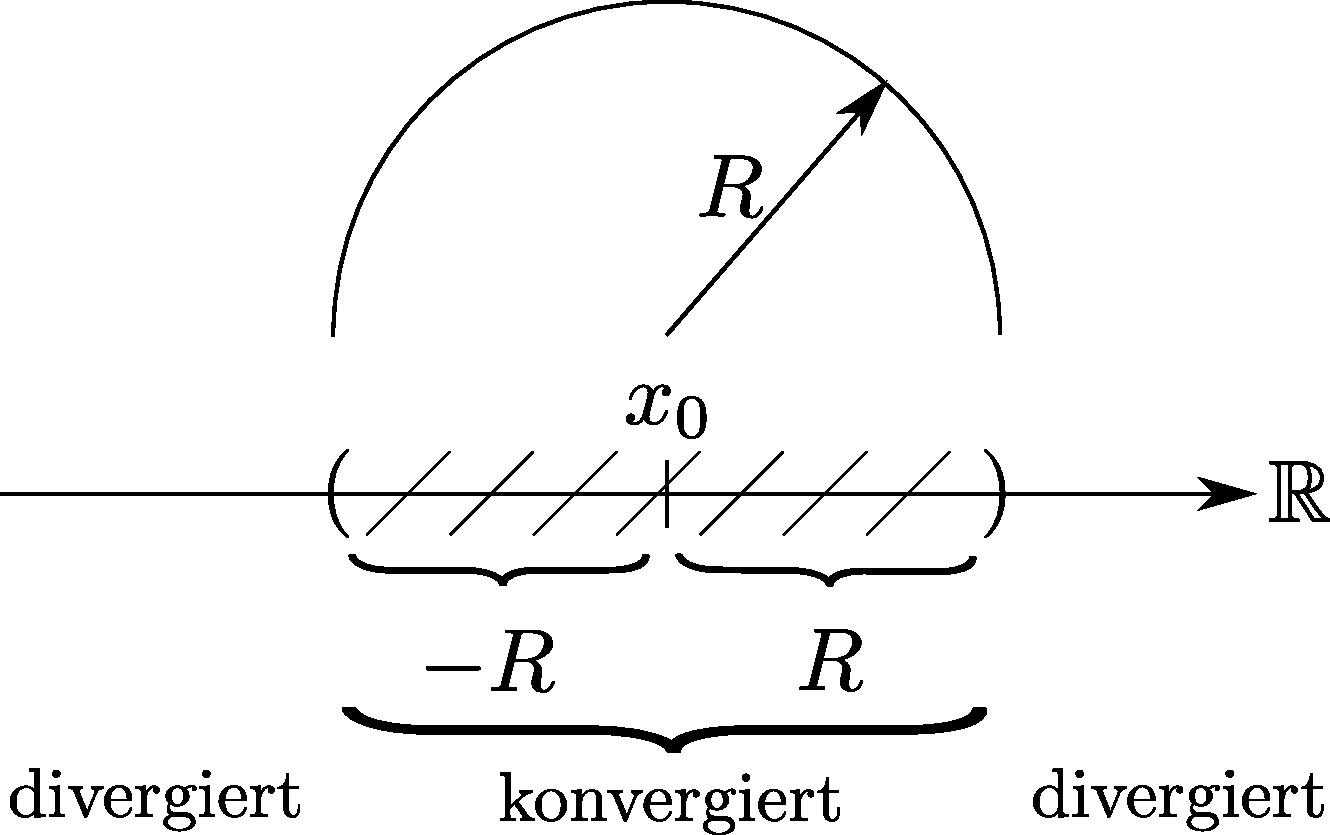
\includegraphics[width=0.6\textwidth]{konvergenzradius.pdf}
\end{figure}

\[ \boxed{ \begin{array}{lll} 
    |x| < R & \Rightarrow & \text{Potenzreihe ist konvergent} \\
    |x| > R & \Rightarrow & \text{Potenzreihe ist divergent} \\
    |x| = R & \Rightarrow & \text{überprüfen was für $x=R$ und $-x=R$ gilt}
\end{array} } \]

\[ \boxed{R = \frac{1}{q} = \lim_{K \rightarrow \infty} \left| \frac{a_K}{a_{K + 1}} \right|} \]
% \quad \quad \text{wobei} \quad \quad a_k = \frac{f^{(K)}(x_0)}{K!} } \]

\subsection{Einfache Funktionen als Taylorreihen}
\[ \boxed{e^x = \sum_{K=0}^{\infty} \frac{x^K}{K!}} \]
\[ \boxed{\sin(x) = \sum_{K=0}^{\infty} \frac{(-1)^K x^{2K+1}}{(2K+1)!}} \]
\[ \boxed{\cos(x) = \sum_{K=0}^{\infty} \frac{(-1)^K x^{2K}}{(2K)!}} \]
\[ \boxed{\cosh(x) = \sum_{K=0}^{\infty} \frac{x^{2K}}{(2K)!}} \]
\[ \boxed{\sinh(x) = \sum_{K=0}^{\infty} \frac{x^{2K+1}}{(2K+1)!}} \]

\subsection{Binomische Reihe}
\[ \boxed{(1 + x)^\alpha = \sum_{K=0}^{\infty}\left(\begin{matrix}\alpha\\K\end{matrix}\right)x^k = \sum_{K=0}^{\infty}\frac{\alpha !}{K! \cdot (\alpha - K)!}x^k} \]

\subsection{McLaurin-Reihe (Taylorreihe mit Entwicklungspunkt $x_0 = 0)$}
Eine Taylorreihe mit Entwicklungspunkt $x_0 = 0$ wird MacLaurin-Reihe genannt
\[ \boxed{f(x) = \underbrace{\sum_{K=0}^{\infty}\frac{f^{(K)}(0)}{K!} x^K}_{\text{Taylorreihe}}} \]
\[ \boxed{f(x) = \underbrace{\sum_{K=0}^{n}\frac{f^{(K)}(0)}{K!} x^K}_{T_{(n,x_0)}(x)} + \underbrace{\sum_{K=n+1}^{\infty}\frac{f^{(K)}(0)}{K!} x^K}_{R_{n+1}(x)}} \]
$T_{(n,x_0)}(x)$ ist dabei das Taylorpolynom vom Grad n und $R_{n+1}(x)$ ist das Restglied. \\
Für das Restglied gilt: Es gibt eine Zahl $\xi$ zwischen $x_0$ und $x$ so, dass gilt:
\[ \boxed{R_{n+1} = \frac{f^{(n + 1)}(\xi)}{(n + 1)!} \cdot (x - x_0)^{n + 1}} \]
Dies ist eine Restgliedformel (Lagrangsche Darstellung für $R_{n + 1}$).


\subsection{Kochrezept Taylorreihen}
\begin{enumerate}
  \item Stelle finden, an welcher die Funktion approximiert werden soll. 
  \item Bereich und Genauigkeit bzw. Fehler definieren oder den Grad der Potenzreihe fix wählen. 
  \item $a_0$, $a_1$, \dots $a_n$ berechnen. $n$ ist dabei der Grad der Potenzreihe
  \item Potenzreihe zusammensetzten
\end{enumerate}

\ifti
\subsection{Taylorreihe mit dem TI-89 berechnen}
\begin{verbatim}
taylor(Funktion,Variable,Ordnung[,Punkt])
\end{verbatim}
Funktion: Funktion, zu welcher die Taylorreihe gesucht ist. \\
Variable: Variable in Funktion\\
Ordnung: Ordnung der Taylorreihe\\
Punkt: Optional: Punkt, an dem Die Funktion approximiert wird. (Default: 0)
\fi
\ifnspire
\subsection{Taylorreihe mit dem TI-Nspire berechnen}
\begin{verbatim}
taylor(Funktion,Variable,Ordnung[,Punkt])
\end{verbatim}
Funktion: Funktion, zu welcher die Taylorreihe gesucht ist. \\
Variable: Variable in Funktion\\
Ordnung: Ordnung der Taylorreihe\\
Punkt: Optional: Punkt, an dem Die Funktion approximiert wird. (Default: 0)
\fi


\chapter{Fourierreihen}
% coding:utf-8



%----------------------------------------

%FOSAMATH, a LaTeX-Code for a mathematical summary for basic analysis

%Copyright (C) 2013, Daniel Winz, Ervin Mazlagic, Adrian Imboden, Philipp Langer



%This program is free software; you can redistribute it and/or

%modify it under the terms of the GNU General Public License

%as published by the Free Software Foundation; either version 2

%of the License, or (at your option) any later version.



%This program is distributed in the hope that it will be useful,

%but WITHOUT ANY WARRANTY; without even the implied warranty of

%MERCHANTABILITY or FITNESS FOR A PARTICULAR PURPOSE.  See the

%GNU General Public License for more details.

%----------------------------------------


% coding:utf-8
\section{Fourierreihen}

\subsection{gerade oder ungerade Funktionen}

\subsubsection{Gerade Funktion: }
\[ \boxed{f(-x) = f(x)} \]
Die Funktion ist an der y-Achse gespiegelt. 
\subsubsection{Ungerade Funktion: }
\[ \boxed{f(-x) = -f(x)} \]
Die Funktion wird am Koordinatenursprung um 180° gedreht. 
\subsubsection{Achtung: }
Wichtig ist dabei, dass die Funktion erst nach der Erweiterung auf ganz $\mathbb{R}$ darauf geprüft wird, ob sie gerade oder ungerade ist. \\
So ist $\sin(x)$ eine ungerade Funktion. Wird jedoch nur die Periode $[0, \pi]$ betrachtet, so ist dies eine gerade Funktion. 

\begin{figure}[h!]
\centering
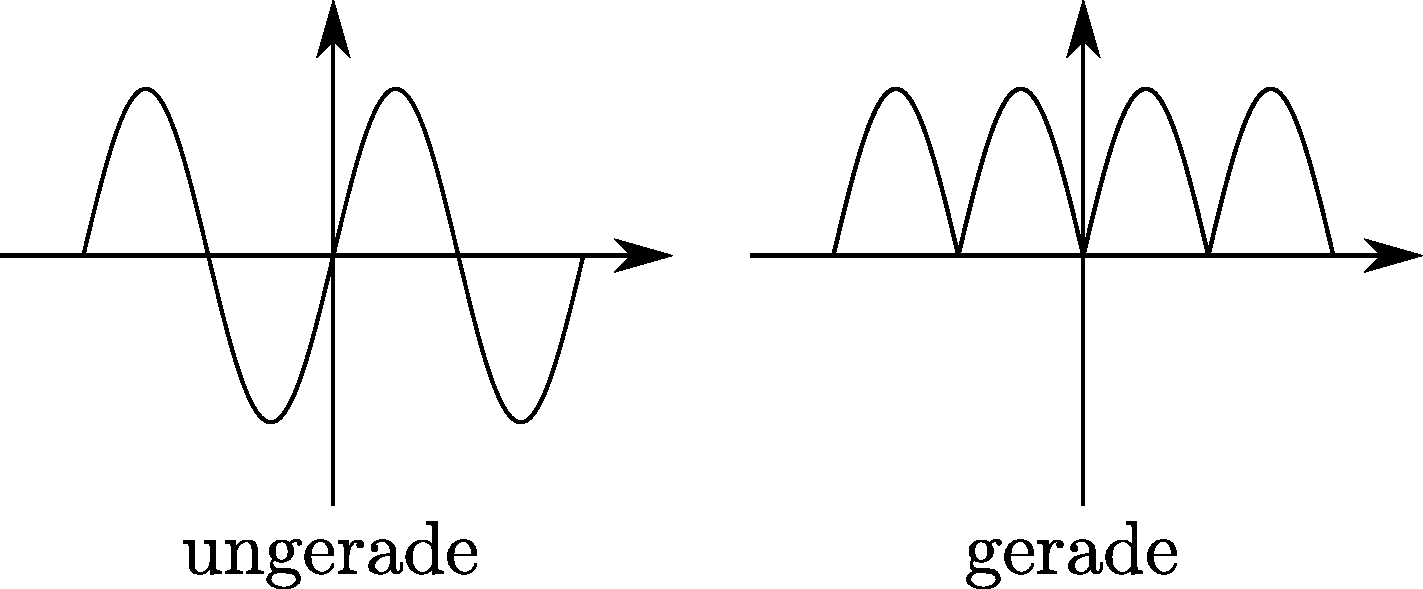
\includegraphics[width=0.7\textwidth]{geradeungerade.pdf}
\end{figure}

\subsection{n-te Partialsumme einer Fourierreihe für die Periode $2\pi$}
Die folgende Fourierreihe besitzt eine Periode von 2 $\pi$. 
\[ \boxed{f_n(x) = \frac{a_0}{2} + \sum_{K=1}^n \left(a_k \cdot \cos(kx) + b_k \cdot \sin(Kx)\right)} \]

\subsection{Koeffizienten für die Periode $2\pi$}
\[ \boxed{a_n = \frac{1}{\pi} \int_0^{2 \pi} f(x) \cos(nx) dx} \]
\[ \boxed{b_n = \frac{1}{\pi} \int_0^{2 \pi} f(x) \sin(nx) dx} \]
\[ \boxed{a_0 = \frac{1}{\pi} \int_0^{2 \pi} f(x) dx
} \]
Ist $f$ eine ungerade Funktion d.h. $f(-x) = -f(x)$, so gilt, da der $\cos(x)$ eine gerade Funktion ist: 
\[ a_k \equiv 0 \quad \forall K\]
\[ a_0 \equiv 0 \]
Ist $f$ eine gerade Funktion: 
\[ b_k \equiv 0 \quad \forall K \]

\subsection{n-te Partialsumme für die Periode T}
\[ \boxed{f_n(x) = \frac{a_0}{2} + \sum_{K=1}^n \left(a_k \cdot \cos \left(\frac{2 \pi}{T} K x\right) + b_k \cdot \sin\left(\frac{2 \pi}{T} K x\right)\right)} \]

\subsection{Koeffizienten für die Periode T}
\[ \boxed{a_n = \frac{2}{T} \int_T f(x) \cos(\frac{2 \pi}{T} K x) dx} \]
\[ \boxed{b_n = \frac{2}{T} \int_T f(x) \sin(\frac{2 \pi}{T} K x) dx} \]
\[ \boxed{a_0 = \frac{2}{T} \int_T f(x) dx
} \]

\subsection{Kochrezept zu Fourierreihen}
\begin{enumerate}
  \item Periode bestimmen
  \item Funktion auf ganz $\mathbb{R}$ fortsetzen
  \item Bestimmung, ob gerade oder ungerade Funktion\\
  f ungerade: $a_0, a_k = 0$\\
  f gerade: $b_k = 0$
  \item $a_0, a_k$ und $b_k$ berechnen
  \item n-te trigonometrische Summe zu f hinschreiben
\end{enumerate}

\ifti
\subsection{Koeffizienzen der Fourierreihe mit dem TI-89 berechnen}
% \verb?integrate(?$\mathtt{\pi}$\verb?/2 * sin(@n1 * x),x,0,?$\mathtt{\pi}$\verb?)?\\
% $\mathtt{integrate\left(\frac{\pi}{2} \cdot sin(@n1 \cdot x), x, 0, \pi\right)}$\\
% $\text{integrate}\left(\frac{\pi}{2} \cdot \sin(@n1 \cdot x), x, 0, \pi\right)$
\verb?integrate(Ausdruck,Variable,untere Grenze, obere Grenze)? \\
\verb?integrate(EXPR,VAR[,LOW,UP])? \\\\
\begin{tabular}{@{}lll}
\verb?EXP?  & Ausdruck      & bezeichnet den Term der die Fourierreihe beschreibt \\
\verb?VAR?  & Variable      & bezeichnet die Variable, nach der integriert wird \\
\verb?LOW?  & untere Grenze & Anfangspunkt der Integration \\
\verb?HIGH? & obere Grenze  & Endpunkt der Integration \\
\end{tabular}\\
Für K wird \verb?@n1? eingegeben. 
\fi
\ifnspire
\subsection{Koeffizienten der Fourierreihe mit dem TI-Nspire berechnen}
\[ \int_{\boxed{0}}^{\boxed{\pi}}\boxed{\frac{\pi}{2}\sin(\mathtt{@n1} \cdot x)}~d\boxed{x} \]
$\mathtt{@n1}$ wird dabei anstelle von K eingegeben. Das $\mathtt{@}$ findet man dabei bei den Symbolen (Taste $\boxed{\boxed{^{\infty \beta ^\circ}}}$)
\fi


\chapter{Komplexe Zahlen}
%n coding:utf-8

%----------------------------------------
%FOSAMATH, a LaTeX-Code for a mathematical summary for basic analysis
%Copyright (C) 2013, Daniel Winz, Ervin Mazlagic, Adrian Imboden, Philipp Langer

%This program is free software; you can redistribute it and/or
%modify it under the terms of the GNU General Public License
%as published by the Free Software Foundation; either version 2
%of the License, or (at your option) any later version.

%This program is distributed in the hope that it will be useful,
%but WITHOUT ANY WARRANTY; without even the implied warranty of
%MERCHANTABILITY or FITNESS FOR A PARTICULAR PURPOSE.  See the
%GNU General Public License for more details.
%----------------------------------------

% coding:utf-8
\section{Definition komplexe Zahlen}
Eine komplexe Zahl ist ein Vektor mit einer Komponente im realen Teil und 
einer Komponente im imaginären Teil. 

\section{Darstellung von komplexen Zahlen}
\subsection{Gausssche Zahlenebene}
Komplexe Zahlen können nicht auf dem Zahlenstrahl abgebilder werden. Daher wird 
dafür die gausssche Zahlenebene eingeführt. Das ist ein Koordinatensystem. Auf 
der x-Achse liegt der normale Zahlenstrahl. Auf der y-Achse wird die imaginäre 
Achse gelegt. 
\begin{center}
\begin{tikzpicture}[domain=-4:4]
  % Raster
  \draw[very thin,color=gray] (-1.9,-0.9) grid (3.9,2.9);
  % x-Achse
  \draw[->] (-2.2,0) -- (4.2,0) node[right] {$Re$};
  % y-Achse
  \draw[->] (0,-1.2) -- (0,3.2) node[above] {$Im$};
  % Linien, Pfeile
  \draw[-latex] (0,0) -- (3,2) node[right] {$a+bj$};
  \draw[-latex] (3,0) -- (3,2);
  \draw[-latex] (0,2) -- (3,2);
  % unabhängige Beschriftungen
  \node at (1.5,2.2) {a};
  \node at (3.2,1) {b};
  % Funktionen
%   \draw[color=red] plot (\x,0.5*\x) node[right] {$f(x) =0.5x$};
%   \draw[color=blue] plot (\x,{sin(\x r)}) node[right] {$f(x) = \sin x$};
%   \draw[color=orange] plot (\x,{0.05*exp(\x)}) node[right] {$f(x) = \frac{1}{20} \mathrm e^x$};
\end{tikzpicture}
\end{center}
Eine komplexe Zahl wird dabei in der Form $a+bj$ dargestellt, wobei 
$a, b \in \mathbb{R}$. 
\[ z = \text{Re} + j \cdot \text{Im} \]
\newpage

\subsection{Polardarstellung}
Bei der Polardarstellung wird eine Komplexe Zahl nicht mehr mittels der realen 
und imaginären Komponenten dargestellt. Stattdessen wird die Position der Zahl 
in der gaussschen Zahlenebene durch den Abstand vom Nullpunkt und den Winkel 
gegenüber der Horizontalen definiert. 
\begin{center}
\begin{tikzpicture}[domain=-4:4]
  % Raster
  \draw[very thin,color=gray] (-1.9,-0.9) grid (3.9,2.9);
  % x-Achse
  \draw[->] (-2.2,0) -- (4.2,0) node[right] {$Re$};
  % y-Achse
  \draw[->] (0,-1.2) -- (0,3.2) node[above] {$Im$};
  % Linien, Pfeile
  \draw[-latex] (0,0) -- (3,2) node[right] {$r \cdot \cis(\varphi)$};
  \draw[-latex] (1,0) arc (0:33.7:1);
  % unabhängige Beschriftungen
  \node at (1.2,0.3) {$\varphi$};
  \node at (1.5,1.3) {$r$};
  % Funktionen
%   \draw[color=red] plot (\x,0.5*\x) node[right] {$f(x) =0.5x$};
%   \draw[color=blue] plot (\x,{sin(\x r)}) node[right] {$f(x) = \sin x$};
%   \draw[color=orange] plot (\x,{0.05*exp(\x)}) node[right] {$f(x) = \frac{1}{20} \mathrm e^x$};
\end{tikzpicture}
\end{center}
\[ \boxed{z = r \cdot \cos(\varphi) + r \cdot j \cdot \sin(\varphi) 
= r \cdot \cis(\varphi)} \]

\subsubsection{Umrechnung Kartesisch $\rightarrow$ Polar}
\[ \boxed{r = \sqrt{x^2 + y^2}} \]
\[ \boxed{\varphi = \arctan{\left(\frac{y}{x}\right)}} \]

\subsubsection{Umrechnung Polar $\rightarrow$ Kartesisch}
\[ \boxed{x = r \cdot \cos(\varphi)} \]
\[ \boxed{y = r \cdot \sin(\varphi)} \]
\newpage

\subsection{Exponentialform}
\[ \boxed{z = r \cdot e^{j \varphi} \qquad , r = ||z|| \geq 0
, -\pi < \varphi \leq \pi, \varphi\text{ im Bogenmass}} \]

\subsubsection{Eulersche Formel}
\[ \boxed{e^{j \varphi} = \cos(\varphi) + j \cdot \sin(\varphi)} \]
\[ \boxed{e^{j \pi} + 1 = 0} \]

\subsection{Konjugiert komplex}
Der konjugiert komplexe Wert einer komplexen Zahl wird durch das Spiegeln an 
der x-Achse erreicht. 
\[ \boxed{\overline{a + b j} = a - b j} \]
\[ \boxed{\overline{r \cdot \cis(\varphi)} = r \cdot \cis(-\varphi)} \]
\[ \boxed{\overline{r \cdot e^{j \varphi}} = r \cdot e^{-j \varphi}} \]
\[ \boxed{\overline{\frac{a}{b-jc}} = \frac{a(b+jc)}{(b-jc)(b+jc)} = \frac{ab+jac}{b^2+jbc-jbc-j^2c^2} = \frac{ab+jac}{b^2+c^2} } \]
\begin{figure}[h!]
\centering
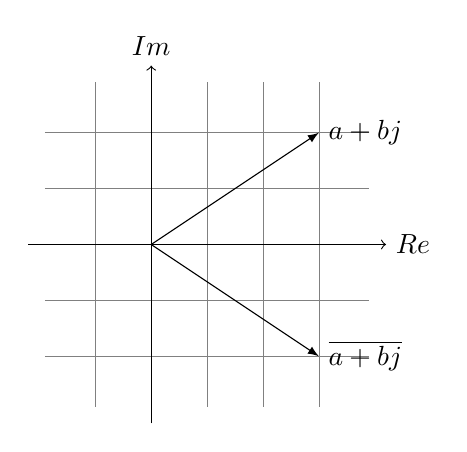
\begin{tikzpicture}[scale=0.71, domain=-4:4]
  % Raster
  \draw[very thin,color=gray] (-1.9,-2.9) grid (3.9,2.9);
  % x-Achse
  \draw[->] (-2.2,0) -- (4.2,0) node[right] {$Re$};
  % y-Achse
  \draw[->] (0,-3.2) -- (0,3.2) node[above] {$Im$};
  % Linien, Pfeile
  \draw[-latex] (0,0) -- (3,2) node[right] {$a+bj$};
  \draw[-latex] (0,0) -- (3,-2) node[right] {$\overline{a+bj}$};
%   \draw[-latex] (0,2) -- (3,2);
  % unabhängige Beschriftungen
  % Funktionen
%   \draw[color=red] plot (\x,0.5*\x) node[right] {$f(x) =0.5x$};
%   \draw[color=blue] plot (\x,{sin(\x r)}) node[right] {$f(x) = \sin x$};
%   \draw[color=orange] 7t plot (\x,{0.05*exp(\x)}) node[right] {$f(x) = \frac{1}{20} \mathrm e^x$};
\end{tikzpicture}
\end{figure}
\newpage

\subsection{Randprobleme}
Möchte man eine komplexe Zahl ermitteln, welche zusammengesetzt mit einer 
anderen Zahl ein bestimmtes Ergebnis ergibt, kann es als sog. 
Randproblem verstanden werden. Diese Randprobleme können graphisch als 
auch analytisch gelöst werden.
\subsubsection{Graphisch}
Grundsätzich geht man von der Form 
\[ ||z-(a+jb)||=r \qquad \Leftrightarrow \qquad||z-a-jb||=r \] 
aus, wobei es statt $\ldots=r$ auch $\ldots\neq r, \ldots>r$
usw. sein kann. Für den graphischen Lösungsweg setzt man das Ergebnis 
nicht als $r$ sondern als $0$ an. So erhält man die komplexe Zahl $z$,
denn dann gilt 
\[ ||z-a-jb||=0 \qquad \Rightarrow \qquad z=a+jb\]
Danach kann $r$ ausgehend von $z$ angewendet werden. Ein $\ldots=r$ beudeutet,
dass alle Lösungen auf einem Kreis liegen mit Mittelpunkt $z$ und Radius $r$. 
Ein $\ldots\leq r$ bedeutet, dass alle Lösungen auf einer Kreisfläche mit
Mittelpunkt $z$ und Radius $r$ liegen usw.
\begin{figure}[h!]
	\centering
	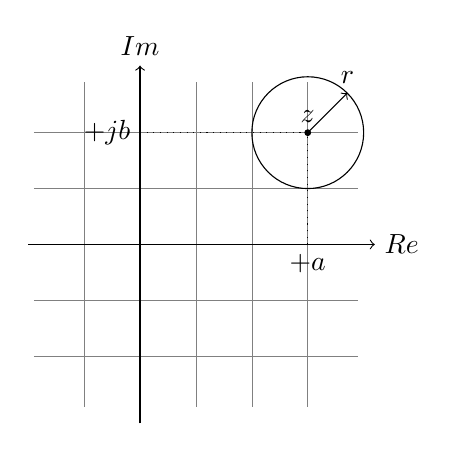
\begin{tikzpicture}[scale=0.71, domain=-4:4]
		\draw[very thin, color=gray] (-1.9, -2.9) grid (3.9, 2.9);
		\draw[->] (-2.0,0) -- (4.2,0) node[right] {$Re$};
		\draw[->] (0,-3.2) -- (0,3.2) node[above] {$Im$};
		\draw[->] (3,2) node[above] {$z$} -- (3.71,2.71) node[above] {$r$};
		\draw[dotted] (3,0) node[below] {$+a$} -- (3,2);
		\draw[dotted] (0,2) node[left] {$+jb$} -- (3,2); 
		\filldraw (3,2) circle (0.05);
		\draw (3,2) circle(1);
	\end{tikzpicture}
	\caption{Randproblem für $||z-(a+jb)||=r$}
\end{figure}

\subsubsection{Analytisch}
Um ein Randproblem analytisch zu lösen kann wie folgt vorgegangen werden.
\begin{itemize}
	\item Gleichung aufstellen \[ ||(a+jb)-(c+jd)||=r \]
	\item Gleichung in die Form $Re+Im=r$ umformen bzw. $j$ isolieren als Faktor
		\[ ||e+j(f+g)||=r \]
	\item Auflösen mit Hilfe der Regel, dass $||e+j(f+g)||$ die Norm,
		also die Länge des Ortsvektors ist und somit gleich 
		$\sqrt{Re^2+Im^2}$ ist.
		\[ \sqrt{e^2+(j(f+g))^2}=r \]
		Durch das Quadrieren fällt der Imaginärteil $j$ weg, denn 
		$j^2=(\sqrt{-1})^2=(-1)$. Somit ergibt sich
		\[ \sqrt{e^2+((-1)(f^2+2fg+g^2))}=r \]
\end{itemize}



\section{Rechenregeln}

\subsection{Addition / Subtraktion}
Komplexe Zahlen werden in der kartesischen Darstellung komponentenweise addiert 
und subtrahiert. 
\[ \boxed{z_1 + z_2 = \text{Re}_1 + \text{Re}_2 + \text{Im}_1 + \text{Im}_2} \]
\[ \boxed{z_1 - z_2 = \text{Re}_1 - \text{Re}_2 - \text{Im}_1 - \text{Im}_2} \]

\subsection{Multiplikation}
Für die Multiplikation / Division von komplexen Zahlen ist es am einfachsten, 
wenn diese in der polaren Darstellung vorliegen. Wenn nicht, müssen sie 
umgeformt werden. 
\[ \boxed{z_1 \cdot z_2 = r_1 \cdot r_2 \cdot \cis(\varphi_1 + \varphi_2)} \]
\[ \boxed{z_1 \cdot z_2 = r_1 \cdot r_2 \cdot e^{j (\varphi_1 + \varphi_2)}} \]

\subsection{Division}
\[ \boxed{\frac{z_1}{z_2} 
= \frac{z_1}{z_2} \cdot \cis(\varphi_1 - \varphi_2)} \]
\[ \boxed{\frac{z_1}{z_2} 
= \frac{r_1}{r_2} \cdot e^{j (\varphi_1 - \varphi_2)}} \]

\subsubsection{Spezialfall}
\[ \boxed{\frac{1}{z} = \frac{1}{r} \cdot \cis(-\varphi)} \]
\[ \boxed{\frac{1}{e^{j \varphi}} = e^{-j\varphi}} \]
\[ \boxed{\overline{r e^{j\varphi}} = r e^{-j\varphi}} \]

% \subsubsection{Geometrisch}
% \begin{tikzpicture}[domain=-4:4]
%   % Raster
%   \draw[very thin,color=gray] (-3.9,-2.9) grid (3.9,2.9);
%   % x-Achse
%   \draw[->] (-4.2,0) -- (4.2,0) node[right] {$Re$};
%   % y-Achse
%   \draw[->] (0,-3.2) -- (0,3.2) node[above] {$Im$};
%   % Linien, Pfeile
%   \draw[-latex] (0,0) -- (3,2) node[right] {$r \cdot \cis(\varphi)$};
%   \draw[-latex] (1,0) arc (0:33.7:1);
%   % unabhängige Beschriftungen
%   \node at (1.2,0.3) {$\varphi$};
%   \node at (1.5,1.3) {$r$};
%   % Funktionen
%    %\draw[color=red] plot (\x,0.5*\x) node[right] {$f(x) =0.5x$};
%    %\draw[color=blue] plot (\x,{sin(\x r)}) node[right] {$f(x) = \sin x$};
%    %\draw[color=orange] plot (\x,{0.05*exp(\x)}) node[right] {$f(x) = \frac{1}{20} \mathrm e^x$};
% \end{tikzpicture}\\

\subsection{Potenzieren}
\[ \boxed{z^n = r^n \cdot \cis(n \cdot \varphi)} 
\qquad \text{Formel von Moivre} \]
\[ \boxed{\left( r e^{j \varphi} \right)^n = r^n \cdot e^{j n \varphi} 
\qquad , n \in \mathbb{Z}} \]

\subsubsection{Potenzgesetze}
\[ \boxed{\begin{array}{l}
z^n \cdot z^m = z^{n +m}\\\\
{(z^n)}^m = z^{n \cdot m}\\\\
z^{-n} = \dfrac{1}{z^n}\\\\
{z_1}^n \cdot {z_2}^n = (z_1 \cdot z_2)^n\\\\
\dfrac{{z_1}^n}{{z_2}^n} = \left(\dfrac{z_1}{z_2}\right)^n
\end{array}} \]

\subsection{Wurzeln}

\subsubsection{Einheitswurzeln}
\[ \boxed{\sqrt[n]{1} = \cis\left(k \cdot \frac{2 \pi}{n}\right) 
\qquad , k = 0, 1, \ldots, n-1} \]

\subsubsection{Allgemeine Wurzeln}
\[ \boxed{\sqrt[n]{z} 
= \sqrt[n]{r}\cis\left(\frac{\varphi}{n} + k \cdot \frac{2 \pi}{n}\right) 
\qquad , k = 0, 1, \ldots, n-1} \]
\[ \boxed{\sqrt[n]{r e^{j \varphi}} 
= \left( r e^{j \varphi} \right)^{\frac{1}{n}} 
= r^{\frac{1}{n}} \cdot e^{\frac{j \varphi}{n} + j \frac{2 \pi}{n}k} 
\qquad , k = 0,\ldots, n - 1} \]

\subsection{Logarithmen}
\[ \boxed{\ln(z) = \ln(r) + j \varphi + 2 \pi k j \qquad , k \in \mathbb{Z}} \]
Hauptwert für $K = 0$
\[ \boxed{\quad \ln(z) = \ln(r) + j \varphi 
\qquad , -\pi < \varphi \leq \pi} \]
